\ifdefined\included
\else
\documentclass[a4paper,11pt,twoside]{StyleThese}
\usepackage{amsmath,amssymb}             % AMS Math
\usepackage[T1]{fontenc}
\usepackage[utf8x]{inputenc}
\usepackage{babel}
\usepackage{datetime}

\usepackage{lmodern}
\usepackage{tabularx}
%\usepackage{tabular}
\usepackage{multirow}

\usepackage{hhline}
\usepackage[left=1.5in,right=1.3in,top=1.1in,bottom=1.1in,includefoot,includehead,headheight=13.6pt]{geometry}
\renewcommand{\baselinestretch}{1.05}

% Table of contents for each chapter

\usepackage[nottoc, notlof, notlot]{tocbibind}
\usepackage{minitoc}
\setcounter{minitocdepth}{2}
\mtcindent=15pt
% Use \minitoc where to put a table of contents

\usepackage{aecompl}

% Glossary / list of abbreviations

\usepackage[intoc]{nomencl}
\iftoggle{ThesisInEnglish}{%
\renewcommand{\nomname}{Glossary}
}{ %
\renewcommand{\nomname}{Liste des Abréviations}
}

\makenomenclature

% My pdf code

\usepackage{ifpdf}

\ifpdf
  \usepackage[pdftex]{graphicx}
  \DeclareGraphicsExtensions{.jpg}
  \usepackage[a4paper,pagebackref,hyperindex=true]{hyperref}
  \usepackage{tikz}
  \usetikzlibrary{arrows,shapes,calc}
\else
  \usepackage{graphicx}
  \DeclareGraphicsExtensions{.ps,.eps}
  \usepackage[a4paper,dvipdfm,pagebackref,hyperindex=true]{hyperref}
\fi

\graphicspath{{.}{images/}}

%% nicer backref links. NOTE: The flag ThesisInEnglish is used to define the
% language in the back references. Read more about it in These.tex

\iftoggle{ThesisInEnglish}{%
\renewcommand*{\backref}[1]{}
\renewcommand*{\backrefalt}[4]{%
\ifcase #1 %
(Not cited.)%
\or
(Cited in page~#2.)%
\else
(Cited in pages~#2.)%
\fi}
\renewcommand*{\backrefsep}{, }
\renewcommand*{\backreftwosep}{ and~}
\renewcommand*{\backreflastsep}{ and~}
}{%
\renewcommand*{\backref}[1]{}
\renewcommand*{\backrefalt}[4]{%
\ifcase #1 %
(Non cité.)%
\or
(Cité en page~#2.)%
\else
(Cité en pages~#2.)%
\fi}
\renewcommand*{\backrefsep}{, }
\renewcommand*{\backreftwosep}{ et~}
\renewcommand*{\backreflastsep}{ et~}
}

% Links in pdf
\usepackage{color}
\definecolor{linkcol}{rgb}{0,0,0.4} 
\definecolor{citecol}{rgb}{0.5,0,0} 
\definecolor{linkcol}{rgb}{0,0,0} 
\definecolor{citecol}{rgb}{0,0,0}
% Change this to change the informations included in the pdf file

\hypersetup
{
bookmarksopen=true,
pdftitle="Évaluation de la sécurité des équipements grand public connectés à Internet",
pdfauthor="Yann BACHY", %auteur du document
pdfsubject="Thèse", %sujet du document
%pdftoolbar=false, %barre d'outils non visible
pdfmenubar=true, %barre de menu visible
pdfhighlight=/O, %effet d'un clic sur un lien hypertexte
colorlinks=true, %couleurs sur les liens hypertextes
pdfpagemode=None, %aucun mode de page
pdfpagelayout=SinglePage, %ouverture en simple page
pdffitwindow=true, %pages ouvertes entierement dans toute la fenetre
linkcolor=linkcol, %couleur des liens hypertextes internes
citecolor=citecol, %couleur des liens pour les citations
urlcolor=linkcol %couleur des liens pour les url
}

% definitions.
% -------------------

\setcounter{secnumdepth}{3}
\setcounter{tocdepth}{2}

% Some useful commands and shortcut for maths:  partial derivative and stuff

\newcommand{\pd}[2]{\frac{\partial #1}{\partial #2}}
\def\abs{\operatorname{abs}}
\def\argmax{\operatornamewithlimits{arg\,max}}
\def\argmin{\operatornamewithlimits{arg\,min}}
\def\diag{\operatorname{Diag}}
\newcommand{\eqRef}[1]{(\ref{#1})}

\usepackage{rotating}                    % Sideways of figures & tables
%\usepackage{bibunits}
%\usepackage[sectionbib]{chapterbib}          % Cross-reference package (Natural BiB)
%\usepackage{natbib}                  % Put References at the end of each chapter
                                         % Do not put 'sectionbib' option here.
                                         % Sectionbib option in 'natbib' will do.
\usepackage{fancyhdr}                    % Fancy Header and Footer

% \usepackage{txfonts}                     % Public Times New Roman text & math font
  
%%% Fancy Header %%%%%%%%%%%%%%%%%%%%%%%%%%%%%%%%%%%%%%%%%%%%%%%%%%%%%%%%%%%%%%%%%%
% Fancy Header Style Options

\pagestyle{fancy}                       % Sets fancy header and footer
\fancyfoot{}                            % Delete current footer settings

%\renewcommand{\chaptermark}[1]{         % Lower Case Chapter marker style
%  \markboth{\chaptername\ \thechapter.\ #1}}{}} %

%\renewcommand{\sectionmark}[1]{         % Lower case Section marker style
%  \markright{\thesection.\ #1}}         %

\fancyhead[LE,RO]{\bfseries\thepage}    % Page number (boldface) in left on even
% pages and right on odd pages
\fancyhead[RE]{\bfseries\nouppercase{\leftmark}}      % Chapter in the right on even pages
\fancyhead[LO]{\bfseries\nouppercase{\rightmark}}     % Section in the left on odd pages

\let\headruleORIG\headrule
\renewcommand{\headrule}{\color{black} \headruleORIG}
\renewcommand{\headrulewidth}{1.0pt}
\usepackage{colortbl}
\arrayrulecolor{black}

\fancypagestyle{plain}{
  \fancyhead{}
  \fancyfoot{}
  \renewcommand{\headrulewidth}{0pt}
}

%\usepackage{MyAlgorithm}
%\usepackage[noend]{MyAlgorithmic}
\usepackage[ED=MITT - STICRT, Ets=INSA]{tlsflyleaf}
%%% Clear Header %%%%%%%%%%%%%%%%%%%%%%%%%%%%%%%%%%%%%%%%%%%%%%%%%%%%%%%%%%%%%%%%%%
% Clear Header Style on the Last Empty Odd pages
\makeatletter

\def\cleardoublepage{\clearpage\if@twoside \ifodd\c@page\else%
  \hbox{}%
  \thispagestyle{empty}%              % Empty header styles
  \newpage%
  \if@twocolumn\hbox{}\newpage\fi\fi\fi}

\makeatother
 
%%%%%%%%%%%%%%%%%%%%%%%%%%%%%%%%%%%%%%%%%%%%%%%%%%%%%%%%%%%%%%%%%%%%%%%%%%%%%%% 
% Prints your review date and 'Draft Version' (From Josullvn, CS, CMU)
\newcommand{\reviewtimetoday}[2]{\special{!userdict begin
    /bop-hook{gsave 20 710 translate 45 rotate 0.8 setgray
      /Times-Roman findfont 12 scalefont setfont 0 0   moveto (#1) show
      0 -12 moveto (#2) show grestore}def end}}
% You can turn on or off this option.
% \reviewtimetoday{\today}{Draft Version}
%%%%%%%%%%%%%%%%%%%%%%%%%%%%%%%%%%%%%%%%%%%%%%%%%%%%%%%%%%%%%%%%%%%%%%%%%%%%%%% 

\newenvironment{maxime}[1]
{
\vspace*{0cm}
\hfill
\begin{minipage}{0.5\textwidth}%
%\rule[0.5ex]{\textwidth}{0.1mm}\\%
\hrulefill $\:$ {\bf #1}\\
%\vspace*{-0.25cm}
\it 
}%
{%

\hrulefill
\vspace*{0.5cm}%
\end{minipage}
}

\let\minitocORIG\minitoc
\renewcommand{\minitoc}{\minitocORIG \vspace{1.5em}}

\usepackage{multirow}
%\usepackage{slashbox}

\newenvironment{bulletList}%
{ \begin{list}%
	{$\bullet$}%
	{\setlength{\labelwidth}{25pt}%
	 \setlength{\leftmargin}{30pt}%
	 \setlength{\itemsep}{\parsep}}}%
{ \end{list} }

\newtheorem{definition}{Définition}
\renewcommand{\epsilon}{\varepsilon}

% centered page environment

\newenvironment{vcenterpage}
{\newpage\vspace*{\fill}\thispagestyle{empty}\renewcommand{\headrulewidth}{0pt}}
{\vspace*{\fill}}

\usepackage{tablefootnote}

\usepackage{hyperref}
\hypersetup{
     colorlinks   = true,
     citecolor    = violet
}
\usepackage{graphicx} % for pdf, bitmapped graphics files
\usepackage{amsmath} % assumes amsmath package installed
\usepackage{amssymb}  % assumes amsmath package installed
\usepackage{bm} % for using bold lowercase greek letters
\usepackage{array}
\usepackage{colortbl}	% to color table background
%\usepackage[table]{xcolor}
\usepackage{subfigure}  
\usepackage{tikz}
\newcommand{\tikzcircle}[2][red,fill=red]{\tikz[baseline=-0.5ex]\draw[#1,radius=#2] (0,0) circle ;}%
\definecolor{turquoise}{rgb}{0.28 1 0.92}
\newcommand{\fratop}[2]{\genfrac{}{}{0pt}{}{#1}{#2}}
\newcommand{\mx}[1]{\mathbf{\bm{#1}}} 				% Matrix symbol
\newcommand{\vc}[1]{\mathbf{\bm{#1}}} 					% Vector symbol
\newcommand{\degree}{\ensuremath{^\circ}}				% define the degree symbol
\newcommand{\pder}[2]{\frac{\partial#1}{\partial#2}}		% partial derivative
\newcommand{\ppder}[2]{\frac{\partial^2 #1}{\partial#2^2}}		% second partial derivative
\newcommand{\refframe}[1]{\mbox{\textless#1\textgreater}}	% to denote a reference frame
%\DeclareMathOperator*{\lexmin}{\text{lex}\!\min}			% lexmin
\DeclareMathOperator*{\minimize}{minimize}				% minimize
\DeclareMathOperator*{\maximize}{maximize}				% maximize
%\DeclareMathOperator*{\argmin}{\arg\!\min}				% argmin
%\DeclareMathOperator*{\argmax}{\arg\!\max}				% argmax
\DeclareMathOperator*{\st}{subject\,to}					% subject to
\DeclareMathOperator*{\dif}{\mathrm{d}}					% d
\DeclareMathOperator*{\half}{\frac{1}{2}}					% one half
\newcommand{\mat}[1]{\ensuremath{\begin{bmatrix}#1\end{bmatrix}}}	% matrix
\newcommand{\rank}[1]{\text{rank}(#1)}							% rank
%\newcommand{\diag}[1]{\text{diag}(#1)}							% diag
\newcommand{\x}{\ensuremath{\times}}
\newcommand{\spac}{\ensuremath{\quad}}						% alias for space in math environment
\newcommand{\dt}[0]{\ensuremath{\Delta t}}					% dt
\newcommand{\dx}[0]{\ensuremath{\delta x}}					% dx
\newcommand{\du}[0]{\ensuremath{\delta u}}					% du
\newcommand{\dhu}[0]{\ensuremath{\delta \hat{u}}}					% \hat{du}
\newcommand{\dbu}[0]{\ensuremath{\delta \bar{u}}}					% \bar{du}
\newcommand{\dtu}[0]{\ensuremath{\delta \tilde{u}}}					% \tilde{du}
\newcommand{\dhx}[0]{\ensuremath{\delta \hat{x}}}					% \hat{dx}
\newcommand{\DX}[0]{\ensuremath{\Delta X}}						% DX
\newcommand{\DU}[0]{\ensuremath{\Delta U}}						% DU
\newcommand{\Ts}[0]{\ensuremath{\top}}							% transpose symbol
\newcommand{\pinv}[0]{\ensuremath{\dagger}}					% pseudoinverse symbol
\newcommand{\Rv}[1]{\ensuremath{\mathbb{R}^{#1}}}				% set of real-valued vectors
\newcommand{\Rm}[2]{\ensuremath{\mathbb{R}^{#1\times #2}}}		% set of real-valued matrices
\newcommand{\Spd}[1]{\ensuremath{\mathbb{S}_+^{#1}}}			% set of symmetric positive-definite matrices
\newcommand{\card}[1]{\ensuremath{\left\vert{#1}\right\vert}}			% cardinality of a set
\DeclareMathOperator{\Tr}{Tr}							% trace
\newcommand{\Expect}{{\rm I\kern-.3em E}}				% expectation
\newcommand{\Normal}{\mathcal{N}}					% normal distribution
\newcommand{\Prob}[1]{\text{P}(#1)}						% probability
\newcommand{\vech}[1]{\text{vech}(#1)}						% vech

\newcommand{\sethree}{\ensuremath{SE(3)}}
\newcommand{\CS}{$\mathcal{CS}$}
\newcommand{\WS}{$\mathcal{WS}$}
\newcommand{\CSfree}{$\mathcal{CS}_{free}$}
\newcommand{\CSobst}{$\mathcal{CS}_{obst}$}
\newcommand{\M}[0]{$\mathcal{M}$}

%\algnewcommand{\algorithmicgoto}{\textbf{go to}}%
%%\algnewcommand{\Goto}[1]{\algorithmicgoto~\ref{#1}}%
%\algnewcommand{\Goto}{\algorithmicgoto\xspace}%
%\algnewcommand{\Label}{\State\unskip}

\newenvironment{definition}[1][Definition]{\begin{trivlist}
\item[\hskip \labelsep {\bfseries #1}]}{\end{trivlist}}

\usepackage{epstopdf}
\usepackage[colorinlistoftodos,prependcaption,textsize=tiny]{todonotes}
\newcommand\explainmore[1]{\textcolor{red}{#1}}
\newcommand\refrephrase[1]{\textcolor{yellow}{#1}}
\newcommand\donerephrasing[1]{\textcolor{green}{#1}}

%DIF PREAMBLE EXTENSION ADDED BY LATEXDIFF
%DIF UNDERLINE PREAMBLE %DIF PREAMBLE
\RequirePackage[normalem]{ulem} %DIF PREAMBLE
\RequirePackage{color}\definecolor{RED}{rgb}{1,0,0}\definecolor{BLUE}{rgb}{0,0,1} %DIF PREAMBLE
\providecommand{\DIFadd}[1]{{\protect\color{blue}\uwave{#1}}} %DIF PREAMBLE
\providecommand{\DIFdel}[1]{{\protect\color{red}\sout{#1}}}                      %DIF PREAMBLE
%DIF SAFE PREAMBLE %DIF PREAMBLE
\providecommand{\DIFaddbegin}{} %DIF PREAMBLE
\providecommand{\DIFaddend}{} %DIF PREAMBLE
\providecommand{\DIFdelbegin}{} %DIF PREAMBLE
\providecommand{\DIFdelend}{} %DIF PREAMBLE
%DIF FLOATSAFE PREAMBLE %DIF PREAMBLE
\providecommand{\DIFaddFL}[1]{\DIFadd{#1}} %DIF PREAMBLE
\providecommand{\DIFdelFL}[1]{\DIFdel{#1}} %DIF PREAMBLE
\providecommand{\DIFaddbeginFL}{} %DIF PREAMBLE
\providecommand{\DIFaddendFL}{} %DIF PREAMBLE
\providecommand{\DIFdelbeginFL}{} %DIF PREAMBLE
\providecommand{\DIFdelendFL}{} %DIF PREAMBLE
%DIF END PREAMBLE EXTENSION ADDED BY LATEXDIFF


\begin{document}


\sloppy
\begin{document}
\fi

\chapter*{Introduction}
\addstarredchapter{Introduction} 
Autonomy is undoubtedly the main goal in Robotics. We just want the robots to be self-reliant and the backing technologies to be as generic as possible. Every incremental research in robotics  directly or indirectly strives to automatize certain processes or mechanisms that solve a problem of physical interaction efficiently and effectively. Though it is controversial to talk about the need of such autonomy in robots, it is an undeniable fact that the research tries to solve robotic problems using algorithms with genericness and self-reliance. Autonomy is not only about the robot having higher awareness about itself and the environment in ideal conditions but the other way around. Developing algorithms with an ability to change, adapt or be flexible is the core problem of establishing autonomy in robots. 

Industrial robots work in static settings and they literally do what it is programmed for specific use-cases, though the robots are flexible enough to be programmed for a variety of tasks. This research work makes an attempt to address these issues that separate both these settings in a profound way with special focus on uncertainties and variability. Lack of precise sensing abilities lead to a variety of uncertainties in scenarios where the robot is mobile or the environment is dynamic. This work focuses on developing smart strategies to improve the ability to handle uncertainties robustly in humanoid and industrial robots. The contributions of this thesis are:
\begin{itemize}
    \item A strategy to model uncertainties of the inertial parameters of a robot for a humanoid robot specific to balancing task scenarios.
    \item A dynamic obstacle avoidance framework proposed for industrial robots equipped with skin sensors for reactivity. 
\end{itemize}

\section{Industrial Robots}
\subsection{History of Industrial Robots}
The idea of automatic machines has been in existence since many centuries with documented illustrations of robots, automata in various interesting applications. Archytas (4th century B.C), the founder of mathematical mechanics, invented an autonomous wooden flying pigeon powered by steam. Fig.~\ref{fig:automatons0} (a) shows this mechanical bird which can fly uninterrupted for hundreds of meters and is considered to be the first ever robot documented. Another interesting application shown in Fig.~\ref{fig:automatons0} (b) is an analog computer (developed during 1st century B.C) that can predict astronomical positions for the purpose of maintaining a calendar and astrological reasons. It has 37 gears enabling the device to track the moon and sun positions keeping track of time. Hydro powered clocks was common in China since the 40th century B.C to study astronomical positions. Fig.~\ref{fig:automatons0} (c) shows Su Song's artistic clock tower developed in 10th century A.D with mechanically controlled mannequins chiming and ringing bells. Al Jazari in the muslim world is known for developing hydro powered automatic machines such as the drink-serving waitress, hand washing automaton, peacock fountain. Though it might look trivial, the works were known for its creative mechanisms, components and design features. Cam \& crank shafts, escapement mechanism in rotating wheels, segmental gears are some of his contributions which are still used in modern mechanical devices today \cite{hill2012book}.  

\begin{figure*}[!tbph]
\begin{subfigure}
[Archytas' bird]{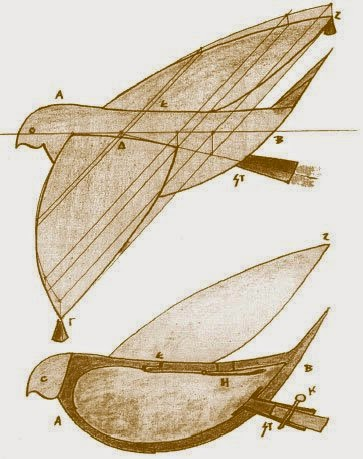
\includegraphics[width=4.1cm,height=5.5cm]{chapters/intro/images/pigionsteam.jpg}}\quad
\end{subfigure}
\begin{subfigure}
[Antikythera mechanism]{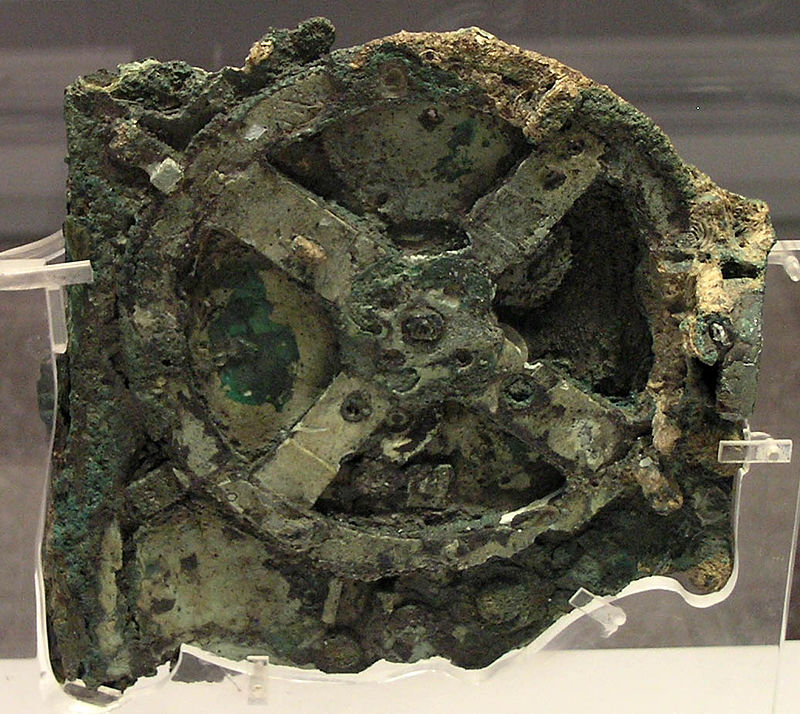
\includegraphics[width=4.3cm,height=5.5cm]{chapters/intro/images/machineanti.jpg}}\quad
\end{subfigure}
\begin{subfigure}
[Su Song's Clock Tower]{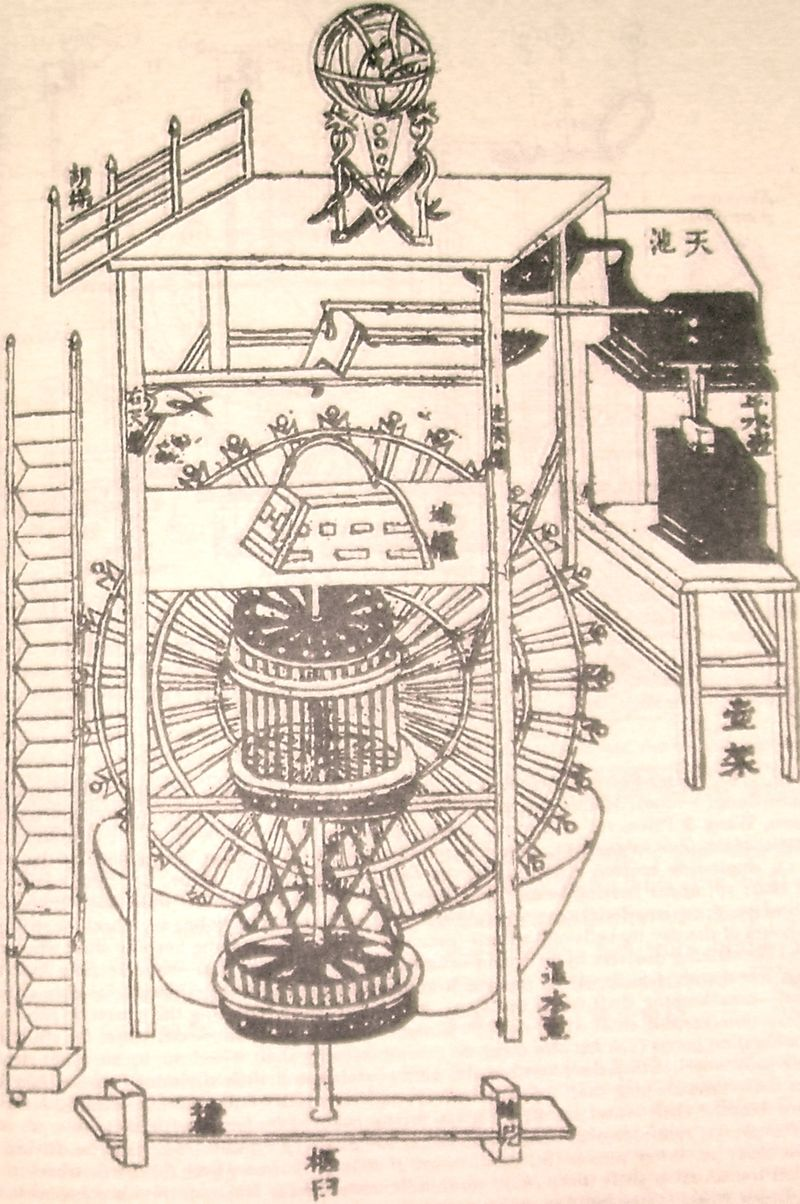
\includegraphics[width=4.1cm,height=5.5cm]{chapters/intro/images/clocktower.JPG}}\quad
\end{subfigure}
\caption{Automatons in the ancient world}
\label{fig:automatons0}
\end{figure*}

Fig.~\ref{fig:automatons1} (a) shows the first ever humanoid robot in the records, designed by Leonardo da Vinci. This mechanical knight has joints similar to human beings with an ability to perform motions such as waving the arms, moving the head and jaws, sitting and standing up. Around 18th century many automatons were developed capable of entertaining, speaking and playing musical instruments. One such musical automaton in the form of an elephant shown in the Fig.~\ref{fig:automatons1} (b) is designed by Hubert Martinet, a french clockmaker in 1774. Another interesting automaton in the Fig.~\ref{fig:automatons1} (c) is the \textit{Digesting Duck} made by Jacques de Vaucanson. This golden mechanical duck imitates the ability to eat and defecate grains.

\begin{figure*}[!tbph]
\begin{subfigure}
[Da Vinci's robot]{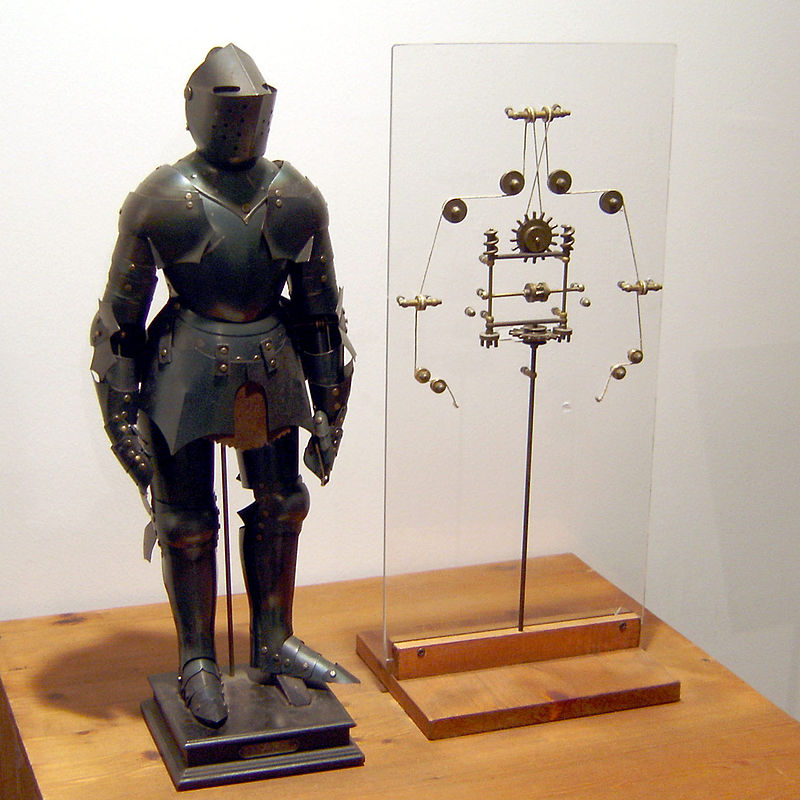
\includegraphics[width=4cm,height=4.5cm]{chapters/intro/images/leorobot.jpg}}\quad
\end{subfigure}
\begin{subfigure}
[Elephant Automaton]{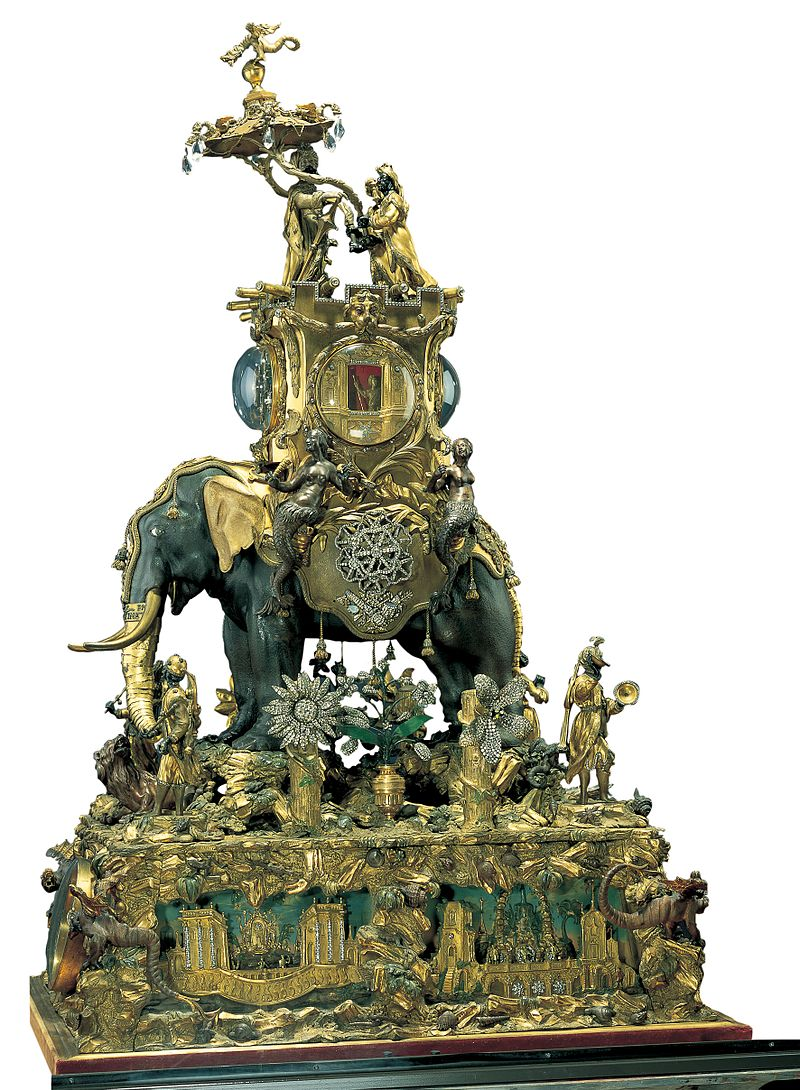
\includegraphics[width=4cm,height=4.5cm]{chapters/intro/images/elephantAutomaton.jpg}}\quad
\end{subfigure}
\begin{subfigure}
[Digesting Duck]{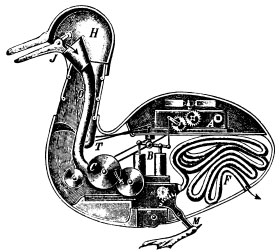
\includegraphics[width=4cm,height=4.5cm]{chapters/intro/images/duck.jpg}}\quad
\end{subfigure}
\caption{Automatons in the 18th Century}
\label{fig:automatons1}
\end{figure*}

% May be talk about Remote-controlled systems

Though most of the automatons were created for fun or artistic satisfaction in the beginning, the characterization of robots to be human look-alike machines that can serve human beings came up in the 20th century. The term \textit{robot} itself was born in 1921 from R.U.R (Rossum's Universal Robots), a czech play written by Karel Čapek. The play depicts robots as good and benevolent workers serving the human beings later gaining super human strength to revolt humans leading to end of life. This negative idea changed after a russian writer, Isaac Asimov made a contrasting characterization of robots as just mechanical creatures with no emotions. Asimov's laws of robotics in 1942 gave way to a new perspective of robots to be seen as an product that could be developed by engineers to improve productivity in manufacturing industries. During the same time period, a programmable mechanism to do spray painting was designed by Pollard and Roselund for DeVilbiss, the first industrial robot supplier. The mechanism is based on pantograph pivoted on two rotary actuators on a fixed base. 


\begin{figure*}[!tbph]
\centering
\begin{subfigure}
[Pollard's Paint Sprayer]{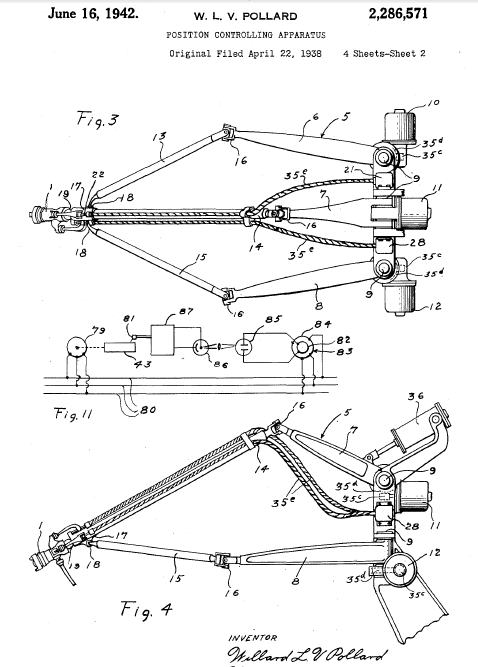
\includegraphics[width=6.5cm,height=6cm]{chapters/intro/images/pollard.png}}
\end{subfigure}
\begin{subfigure}
[Unimate Robot's Television Appearance]{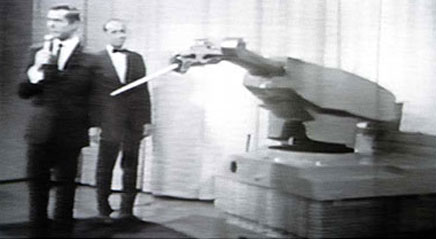
\includegraphics[width=6.5cm,height=6cm]{chapters/intro/images/unimate.jpg}}
\end{subfigure}
\caption{Robotic Mechanisms in the Beginning}
\label{fig:robotmechanisms}
\end{figure*}


In 1954, George Devol developed the the first truly programmable robot UNIMATE which originally consisted of an arm and a drum memory box with pre-programmed tasks. A collaboration with Joseph Engelberger, the father of robotics gave birth to \textit{Unimation}, the first company to make robots which were used to transport and weld die castings on auto bodies preventing humans from dangerous working conditions. Though the numerically controlled turning \& milling machines and the hydraulic assembly machines were programmable, the industrial robots differed in the sophistication of reprogrammability and the versatility to be used for different tasks. This is purely because of the invention of digital computers and integrated circuit technology which allowed to develop the brains of industrial robots.

\begin{figure}[h]
\centering
{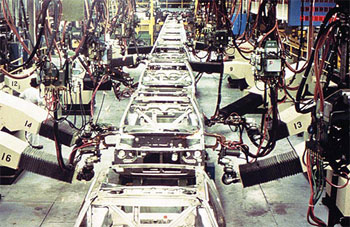
\includegraphics[scale=1]{chapters/intro/images/gm.jpg}}
\caption{Manufacturing unit in General Motors with 'Unimate' robots in 1969}
\label{fig:unimate}
\end{figure}

Ford director Del Harder's interest to install 2000 unimation robots triggered American manufacturing industries to pay attention to the robotics industry a bit more seriously. Installations in General Motors in Ohio, US in the beginning of 1960s marks the real beginning of industrial robotics. After an intense research and development during the next 15 years and the introduction of micro-processors provided the basis for low cost control systems. A norwegian company \textit{Trallfa} designed and developed a cost-effective alternative to Unimate robots for spray painting applications. Several companies such as \textit{Electrolux, ESAB, Atlas Copco,} and \textit{ASEA} followed the same path designing in house robots for their own purposes which suited the requirements of other customers resulting in a product of its own. This phenomenon gave birth to more than 70 robot manufacturers by the year 1973.



The industrial robots were hydraulic or pneumatic in the beginning though they are very suitable for heavier loads. Vicarm in 1968 turned out to be the first electric robot to suit the lighter loads of assembly lines and arc welding. The 6 degree of freedom robot (5 revolute + 1 prismatic) was designed with simplified analytic solutions by Victor Scheinman allowing the robot to track arbitrary paths in the work space of the robot. Cincinnati Milacron, the largest machine tool constructor during the 1970s developed the "The Tomorrow Tool", the first microcomputer based robot. The robots in the beginning were used for simple tasks such as pick and place with no external sensing. External sensing along with the ability of robots to perform advanced motion behaviors gave rise to complex applications like welding, grinding and deburring. The applications can be divided to three main categories: Assembly lines, process operations and material handling. The main motivation of industrial robotics is to apply productive, cost-effective and human safe automation solutions without compromising on the quality of the products. 


The capabilities of robots were purely driven by the manufacturing industries with different industries focusing on different requirements. Material handling required robots of increased loading capacity while arc welding and motion dependant applications required the robot to have better electrical motors and path control. In the beginning of 1980s the assembly lines were mostly focused and shorter cycle time has always been the goal which required robots to be highly dynamic and repeatable. Metal industries required the robots to be very stubborn to work in hot and unsafe working environments. Though robots had complex applications, simple applications such as picking and placing, material transportation were economical for automization. 
These customer demands provided way to the industrial robotic revolution in the 1980s. 


\begin{figure}[!tbph]
\begin{subfigure}
[The Tomorrow Tool-T3]{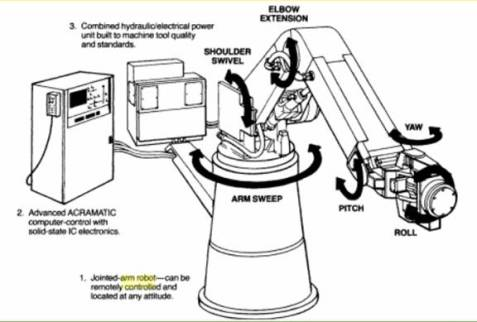
\includegraphics[width=4.3cm,height=6cm]{chapters/intro/images/t3.jpg}}\quad
\end{subfigure}
\begin{subfigure}
[Shakey]{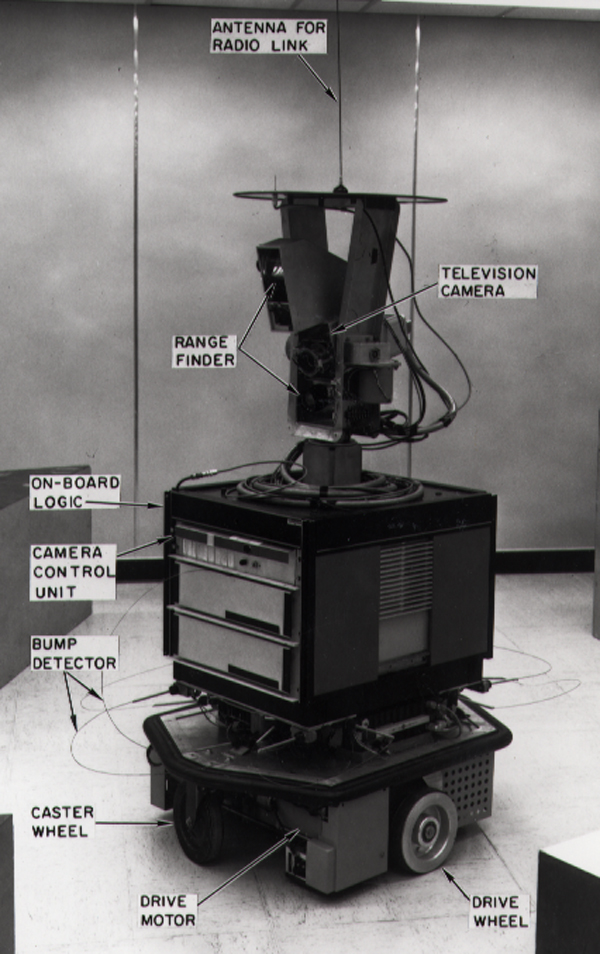
\includegraphics[width=4.1cm,height=6cm]{chapters/intro/images/Shakey.jpg}}\quad
\end{subfigure}
\begin{subfigure}
[Stanford Arm]{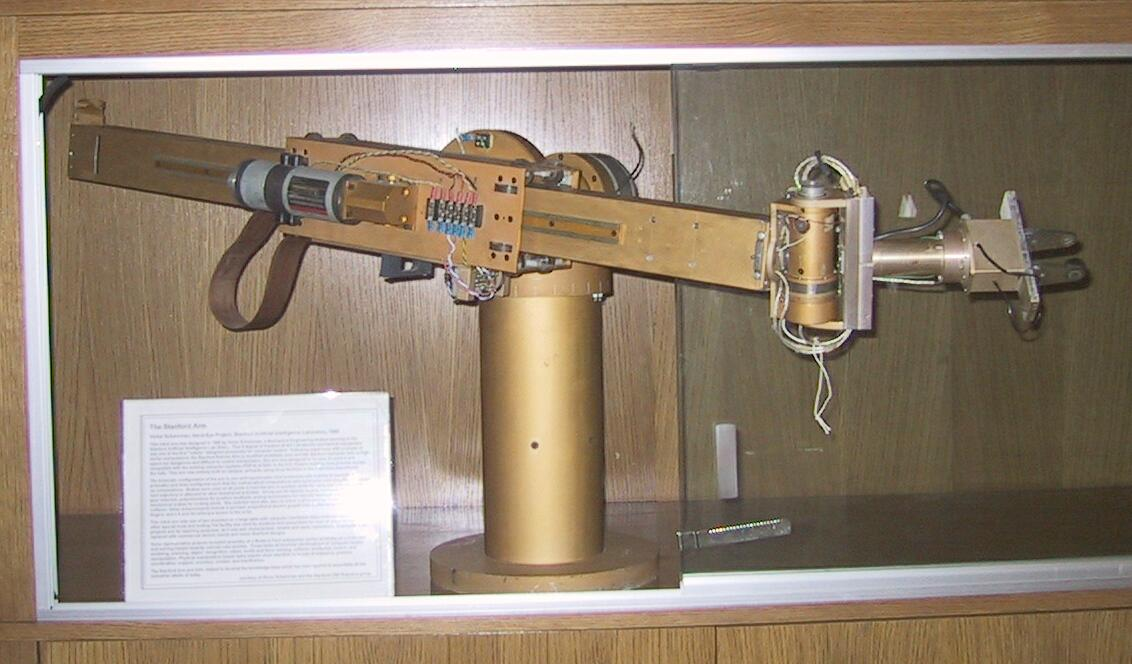
\includegraphics[width=4.1cm,height=6cm]{chapters/intro/images/stanfordarm.JPG}}\quad
\end{subfigure}
\caption{Automatons in the ancient world}
\label{fig:robots}
\end{figure}

Robotics was unanimously accepted as a key focus area to increase industrial development and achieve competitive edge. Advanced sensors such as force sensors, vision cameras and laser scanners were introduced in the late 1980s
to make physical interactions with the environment to improve the intelligence. It is necessary to make deeper connections with the control system to make intelligent decisions in the working environment. Though the vision of robotics in the 1980s was very ambitious to automise factories completely with robots and less human labour, it was very soon realized that robotics being a multi-disciplinary technology is not so easy and certain human work mechanisms are difficult to be replicated. Heterogenous integration of complex systems involves a lot of problems and developing a robotic workcells are more expensive than the workers themselves though they are economically feasible for simpler tasks.

Productivity is a complex concept and the idea of robots solely responsible for improving productivity changed in the beginning of 1990s. The dependence on robotics for more ambitious tasks started to decrease though it was and still an inevitable part of the mechatronic technology to automize and improve productivity. Now robotics are used for medical applications, service, entertainment and disaster handling applications. Though the industrial robots have been in use for quite a long time, there are many challenges not addressed until now. This is where the 'Factory in a Day' project comes into picture.

\subsection{'Factory in a Day' project}
We are aware that robot automation has been into existence since the 1960s and has seen a lot of technological advancements but they are still challenged by installation time and cost involved in setting up robots specific to the functional needs in factories. There is a lot of risk involved in such investment making it economically less attractive to smaller companies. Moreover, the factory setups are fixed environments with hard coded settings of millimeter precision so that they are perfectly under control at all times. Floating robot bases introduces errors and uncertainties which requires more robust components to handle factory scenarios. There is also a big concern in safety of human beings working in robot environments. Though recent technologies are focused towards collaborative robot control where human beings and robots can work together, these algorithms are either completely not matured to be used in factories or not yet known in the industrial community. This thesis is funded by Factory-in-a-Day project which focuses on these issues mentioned above.

Factory-in-a-Day project puts forward the idea of minimizing the installation time and the cost involved from several months to just a single day. The project focuses on the following aspects of robotics which is synonymous to the steps taken in a day to install a robotic setup. 

\begin{itemize}
\item Standardized procedures to design 3D printed custom parts which are usually attached with an existing robot arm and grippers using novel templates to minimize the time taken.
\item The flexibility to be placed in factories without any alteration where intelligent self-calibration and an adaptive framework that helps to connect with the existing machineries in ease.
\item Use rapid teaching to program production tasks in the setup from a rich set of learnable skills
for applications like mould finishing, welding and assembly.
\item Visually intuitive tools for the workers in the factory to assess robot's behavior motion behaviors. Augmented reality can be used to visualize the robot's intended path by wearing a glass to be aware of its activity to be collaborative in nature.
\item A mature human-robot interaction framework to allow the humans collaborate with robots in an unfenced workspace using a dynamic obstacle avoidance framework with proximity skin sensors and 
reactive path planning and control algorithms.
\end{itemize}
The above aspects along with proposed certification procedures and a complete focus on manufacturing industry can radically change the automation sector. The work done in this thesis orients in the direction of the last aspect which is human-robot collaboration. The Fig.~\ref{fig:doa_motivation} (a) shows the reality of many robotics based manufacturing units with fences avoiding dangerous accidents with human beings. There are strict protocols followed to get inside the fence incase of repairs needed. It is definitely not productive, and the new age robot manufacturers such as \textit{Universal Robots} focus on manufacturing robots with safe touch control which allows the robot to stop when the human is in contact. In case the robots are moving fast, they can be programmed to adapt/reduce the speed by monitoring the presence of human beings using laser scanners. Though there are systematic hacks available, the thesis supports the idea of human-robot collaboration in the real sense where they share the workspace with more awareness about the environment and task scenarios. 
\begin{figure}[!tbph]
\begin{subfigure}
[Fenced Robot for Safety]{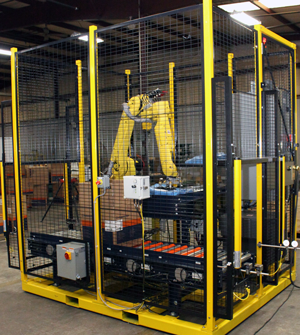
\includegraphics[width=6.6cm,height=6cm]{chapters/intro/images/fencedrobot.png}}\quad
\end{subfigure}
\begin{subfigure}
[New Gen Universal Robot]{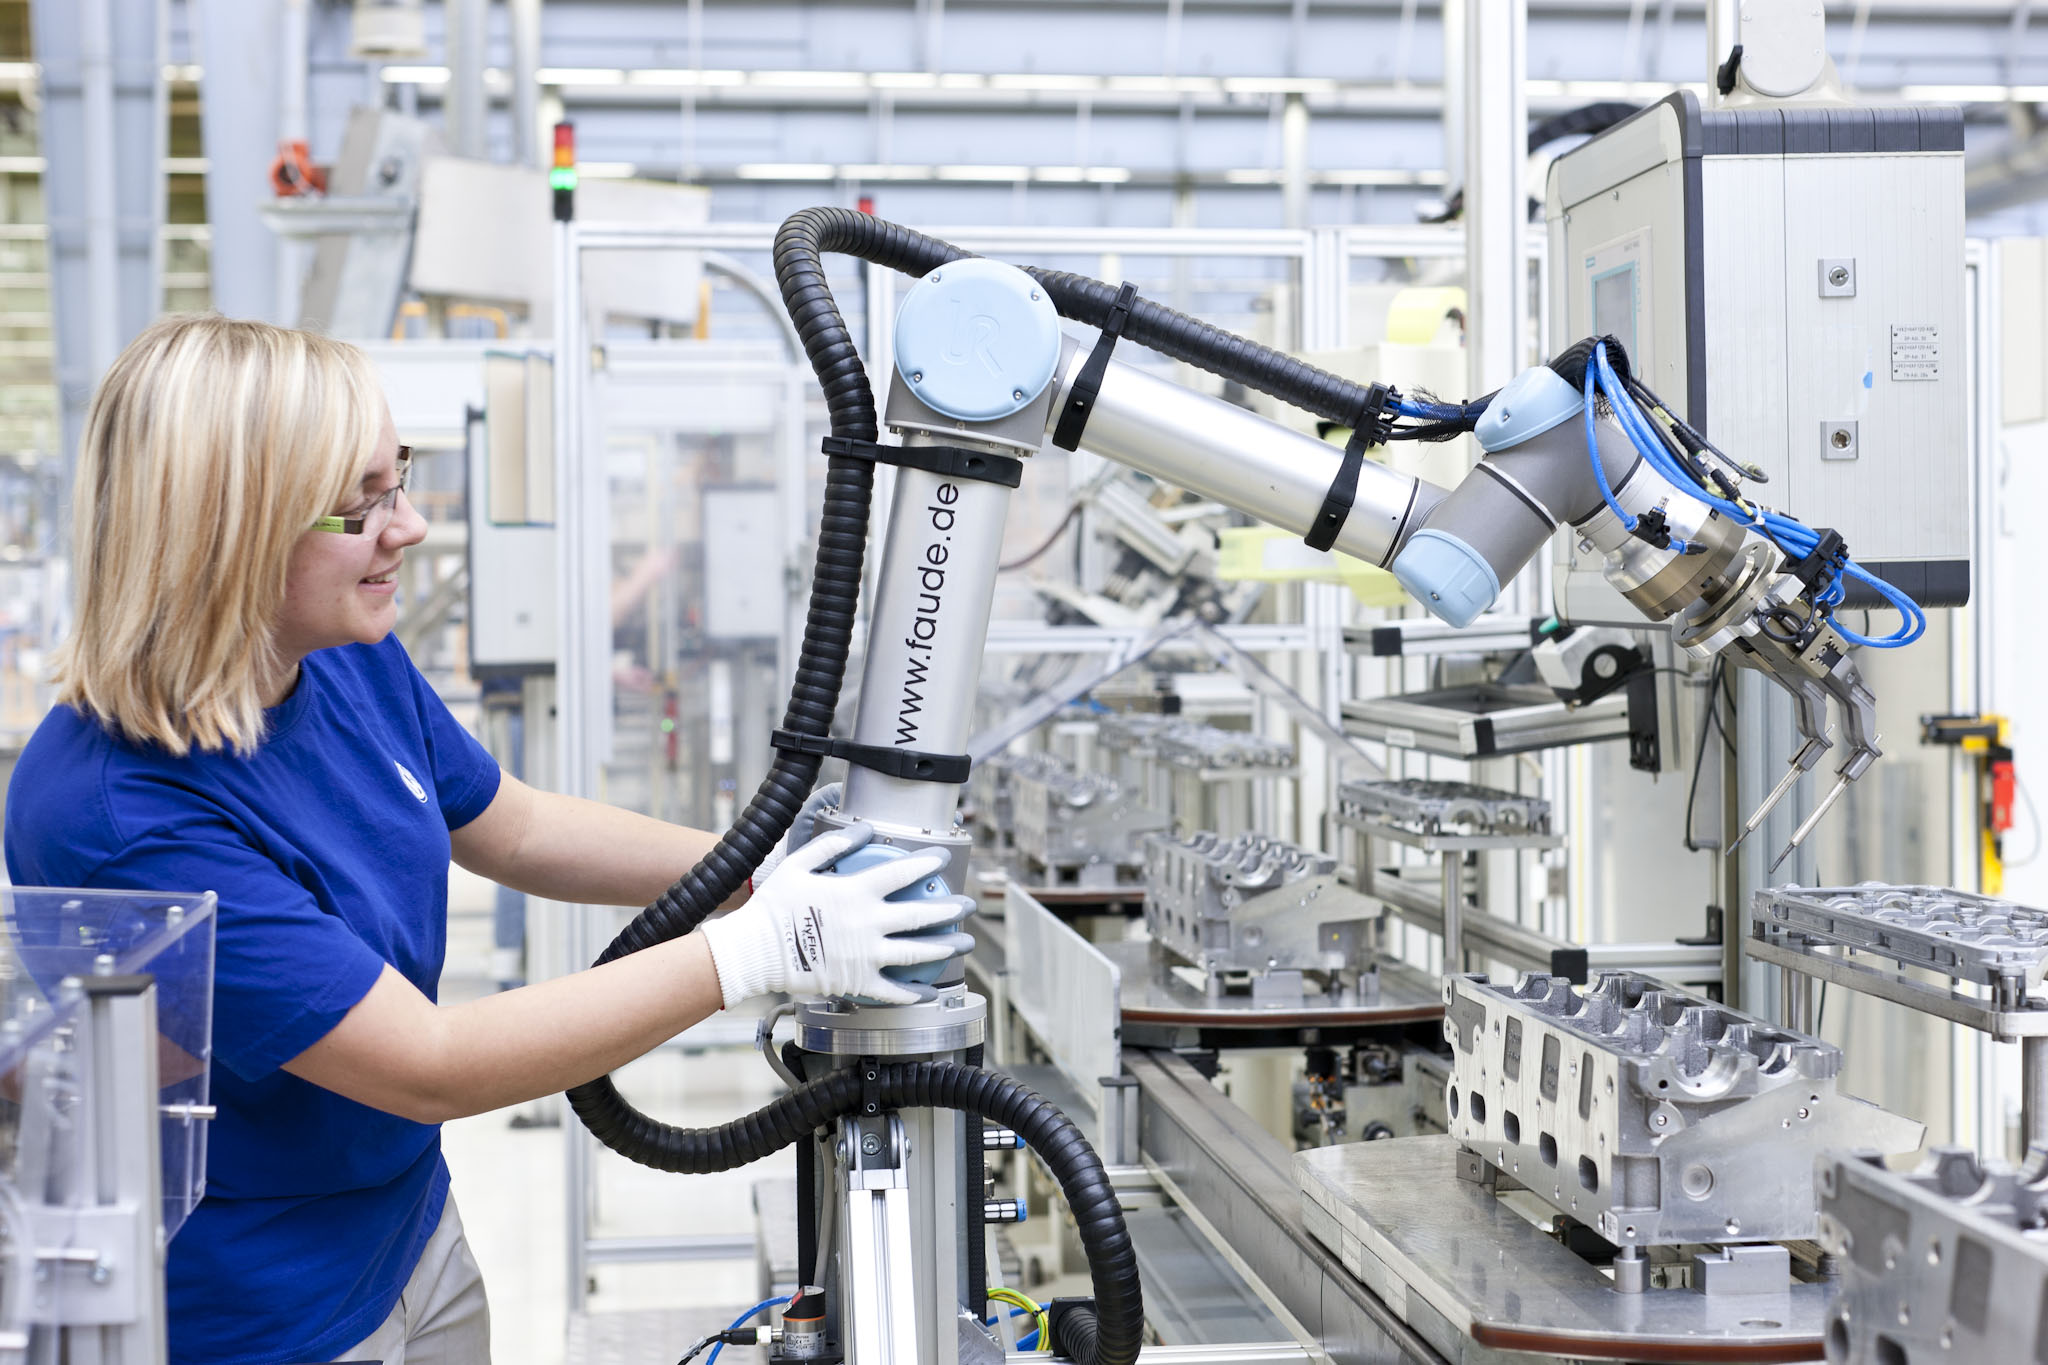
\includegraphics[width=6.5cm,height=6cm]{chapters/intro/images/urcorobot.jpg}}\quad
\end{subfigure}
\caption{Motivation towards Collaborative Robots}
\label{fig:doa_motivation}
\end{figure}


\section{Humanoid Robots}
Humanoid Robots are robotic mechanisms resembling the kinematics of human beings with a head and a torso bridging two arms \& two legs. There are many variants modeling only certain parts of the human body though we stick with the context of legged robots with arms through out this report. Building humanoid robots require the need of understanding human behaviors and kinematic structure deeply. Attempting to build such robots sometimes give us better understanding of human beings making the knowledge flow between both the domains bi-directional. The anthropomorphic design of humanoids also help in getting the acceptance of people as a social entity making the human-robot interaction feasible \cite{fink2012anthropomorphism}. Also the physical ability of humanoids make them suitable for rescue or disaster handling scenarios. The social acceptance and the physical ability of humanoids make them a very good platform to invest on researching technologies that improve the intelligence of such robots.

\subsection{History of Humanoid Robots}
Humanoid robots were just controlled using traditional joint position control methodologies like in industrial robots though there is a need for stiff drive train for precision. WABOT-1 was the first humanoid robot to walk, communicate, visually recognize objects and manipulate them. The robot was built by Kato's lab from University of Waseda in 1973 \cite{kato1973development}. The same lab lead a series of developments achieving the latest one WABIAN-2 which can walk with stretched knees \cite{ogura2006development}. Chronologically WABOT-1 was followed by P2, the first robot to perform stable walking, was launched in 1996 by Honda after 10 years of modular and systematic research focused on dynamic biped walking and stability control \cite{hirai1998development}. The next version P3  was much lighter and gave way to the launch of the famous ASIMO robot in 2000 with a more friendly appearance and improved intelligence \cite{hirose2007honda}. ASIMO's impressive capabilities attracted the attention of robotics researchers and created a perspective of humanoid robots to be exploited for service robotics \cite{kaneko2009cybernetic}. 


\begin{figure}[!tbph]
\begin{subfigure}
[WABOT-1]{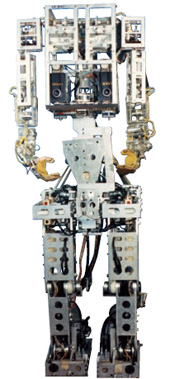
\includegraphics[width=4.1cm,height=6cm]{chapters/intro/images/wabot1.jpg}}\quad
\end{subfigure}
\begin{subfigure}
[ASIMO]{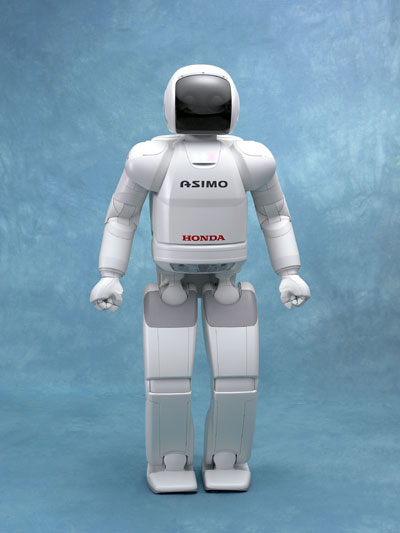
\includegraphics[width=4.2cm,height=6cm]{chapters/intro/images/asimo.jpg}}\quad
\end{subfigure}
\begin{subfigure}
[Kobian]{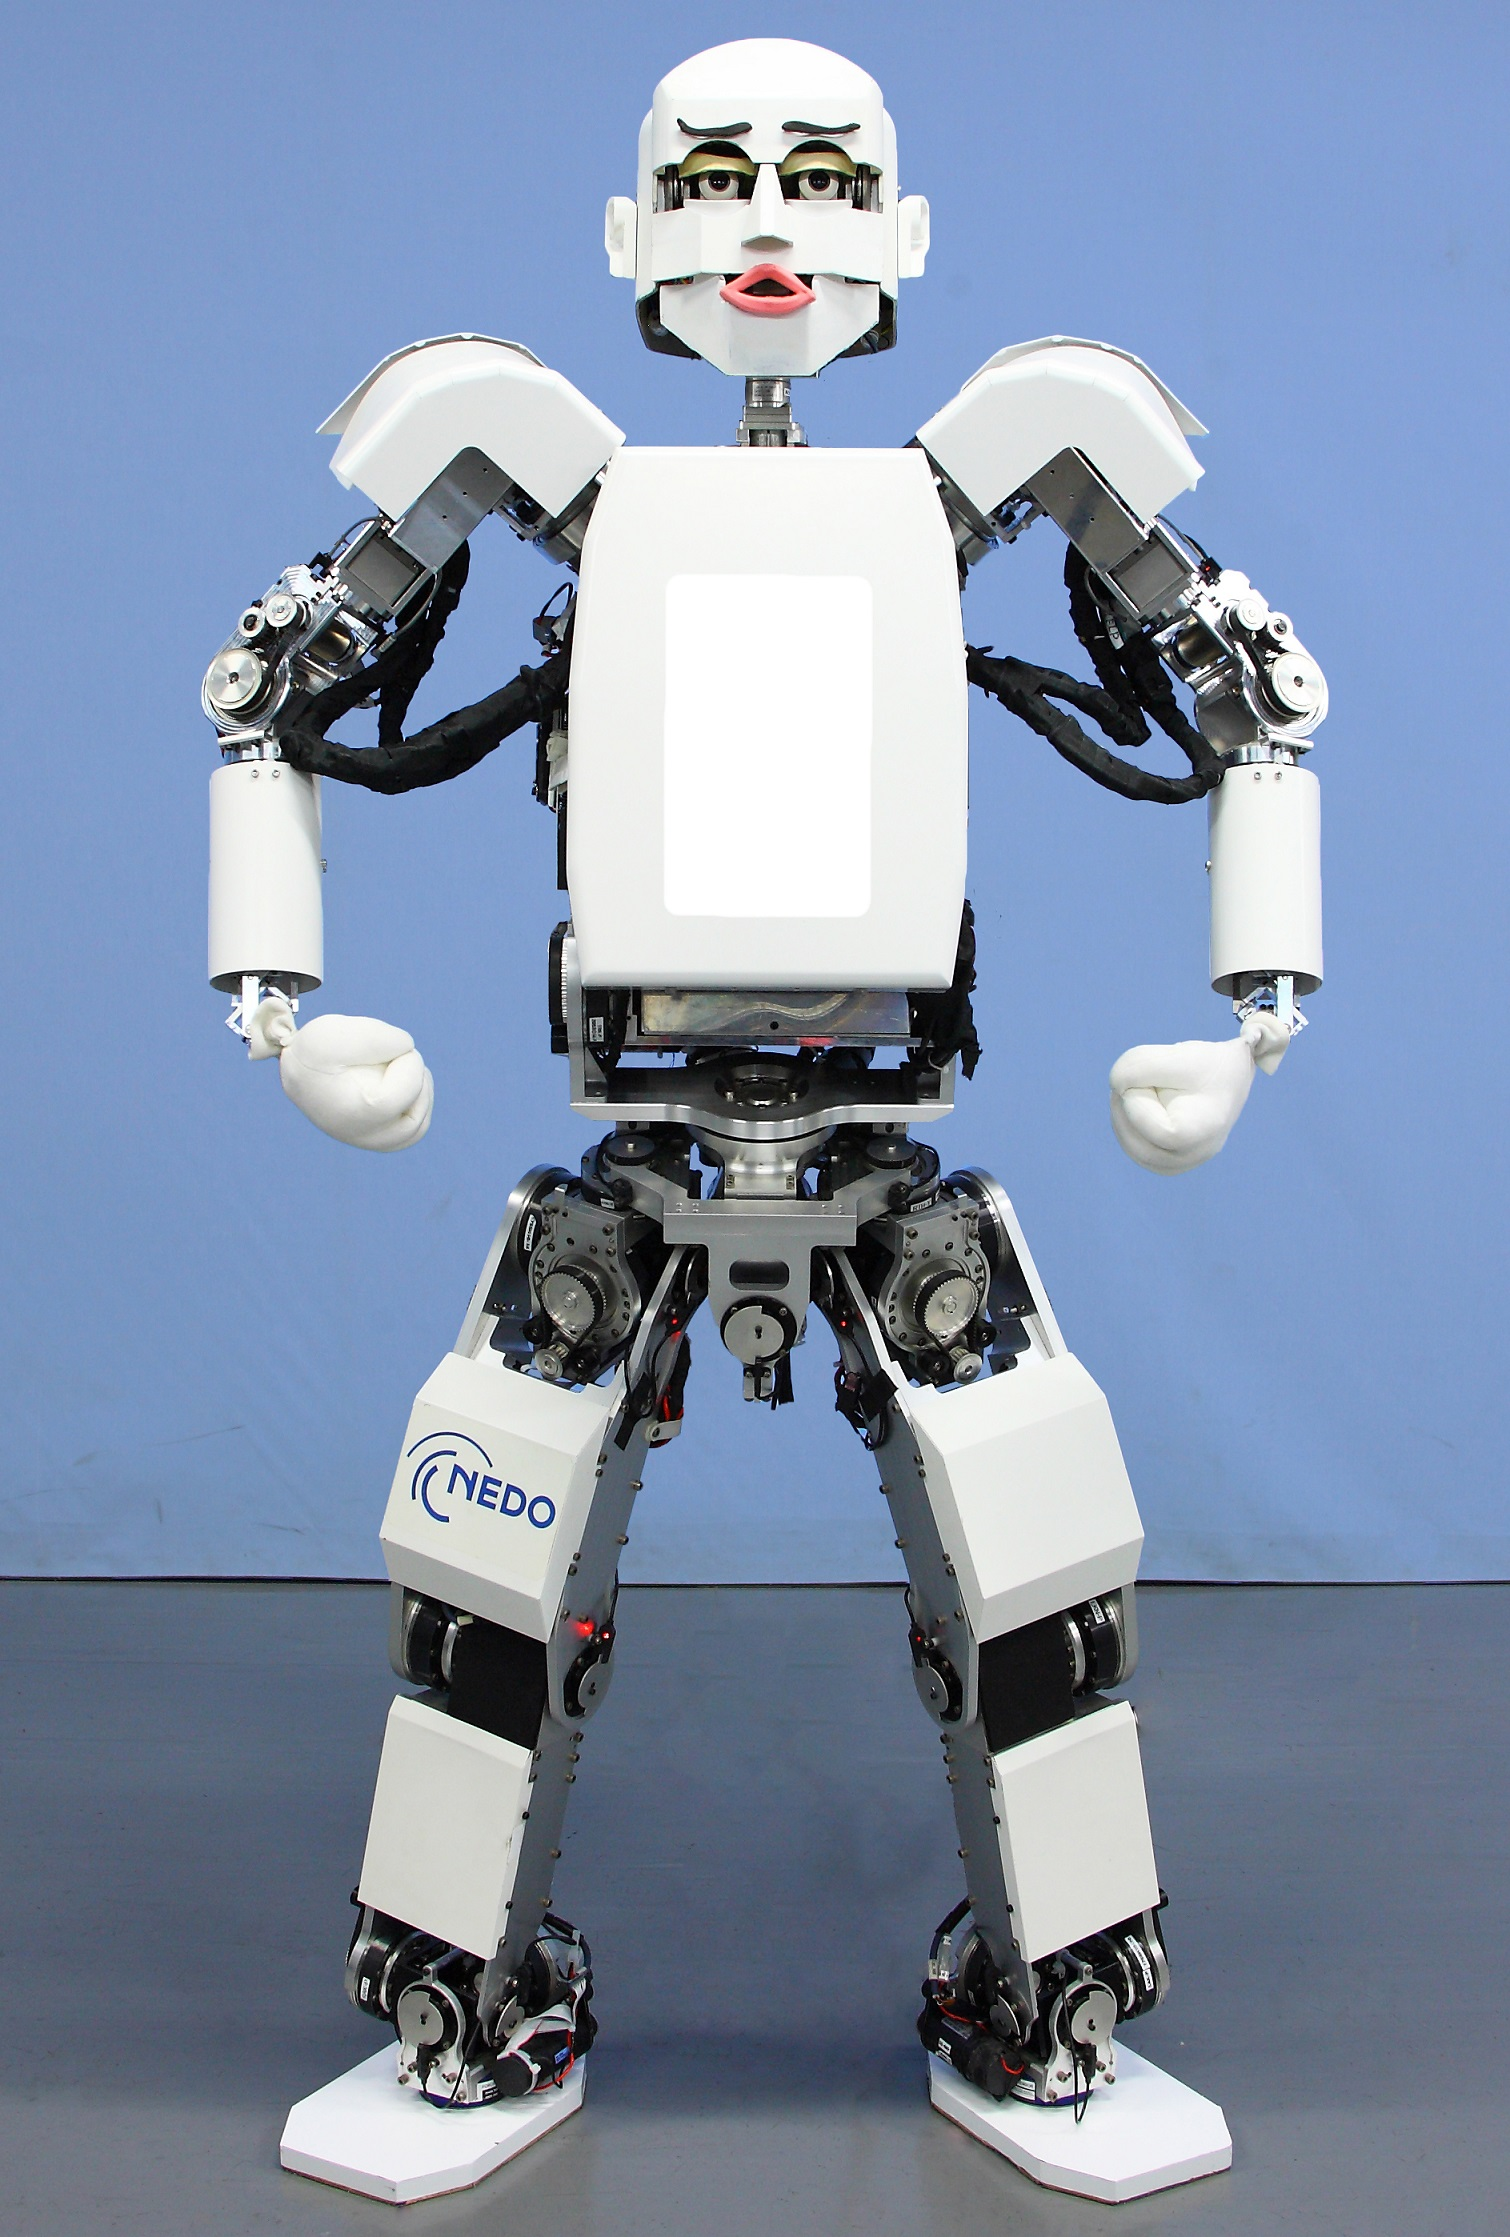
\includegraphics[width=4.2cm,height=6cm]{chapters/intro/images/kobian.jpg}}\quad
\end{subfigure}
\caption{Humanoids of the first generation}
\label{fig:hr_first}
\end{figure}


Japan took the trigger seriously and many humanoids were developed in the last decade both for entertainment and demonstrating physical capabilities. Different sized humanoids with great capabilities were built within the \textit{Humanoid Robotics Project} by Kawada Industries and Japanese National Institute of Advanced Industrial Science and Technology (AIST)  with the first prototype HRP-2P launched in 2002 \cite{kaneko2002design} followed by HRP-2 \cite{Kaneko04humanoidrobot}, HRP-3 \cite{kaneko2008humanoid} in the next years. HRP-4C in 2009 \cite{kaneko2009cybernetic}, assumes a feminine appearance while the latest HRP4 in 2010, is more athletic and light \cite{kaneko2011humanoid}. Sony launched QRIO (previously called SDR-3X), a small humanoid robot for entertainment in 2004 \cite{geppert2004qrio}. Fujitsu Automation also launched a series of small humanoid robots HOAP with the latest version HOAP-3 released in 2005. Other japanese robots include H7  from the University of Tokyo \cite{nishiwaki2007experimental}, Kenta, a musculo-skeletal robot \cite{inaba2003building}, Kojiro in 2007 \cite{mizuuchi2007advanced},Kenshiro in 2012 \cite{nakanishi2012design}. Schaft launched one of the most powerful humanoid robots inspired from HRP-2 series robots in 2013.

The Korea Advanced Institute of Science and Technology (KAIST) invested in developing several versions of KAIST humanoid robots(KHR) since 2002 with the latest one released in 2011 with the name HUBO 2 \cite{kim2002development,park2005mechanical,park2005development,grey2013multi}. The other well known network based robots from Korea are the MAHRU and AHRA series \cite{you2005network,kwon2007biped, kim2011providing}. Technical Unversity of Munich (TUM) built the humanoid robot Johnnie \cite{gienger1999design} followed by an improved version called Lola \cite{lohmeier2009humanoid} known for its fast and robust motions. The Italian Institute of Technology (IIT)  built a torque controlled iCub \cite{metta2010icub} and COMAN in 2012
\cite{tsagarakis2013compliant}. The University Carlos III from Spain, built the Rh-1 in 2007 \cite{arbulu2007real} and its successor TEO in 2011 \cite{monje2011full}. Pal Robotics also built the humanoid robots REEM-B \cite{tellez2008reem}, REEM-C, a human friendly design in 2014 \cite{robotics2014reem}. In 2007, Aldebaran Robotics, a french company launched Nao, one of the most popular small humanoid robot in the world motivated several laboratories to do research on humanoids with less investment \cite{gouaillier2009mechatronic}. The same company presented a torque controlled child-size robot Romeo. 

\begin{figure}[h]
\begin{subfigure}
[HRP2]{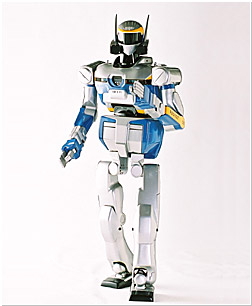
\includegraphics[width=4.4cm,height=6cm]{chapters/intro/images/hrp2.jpg}}\quad
\end{subfigure}
\begin{subfigure}
[Kojiro]{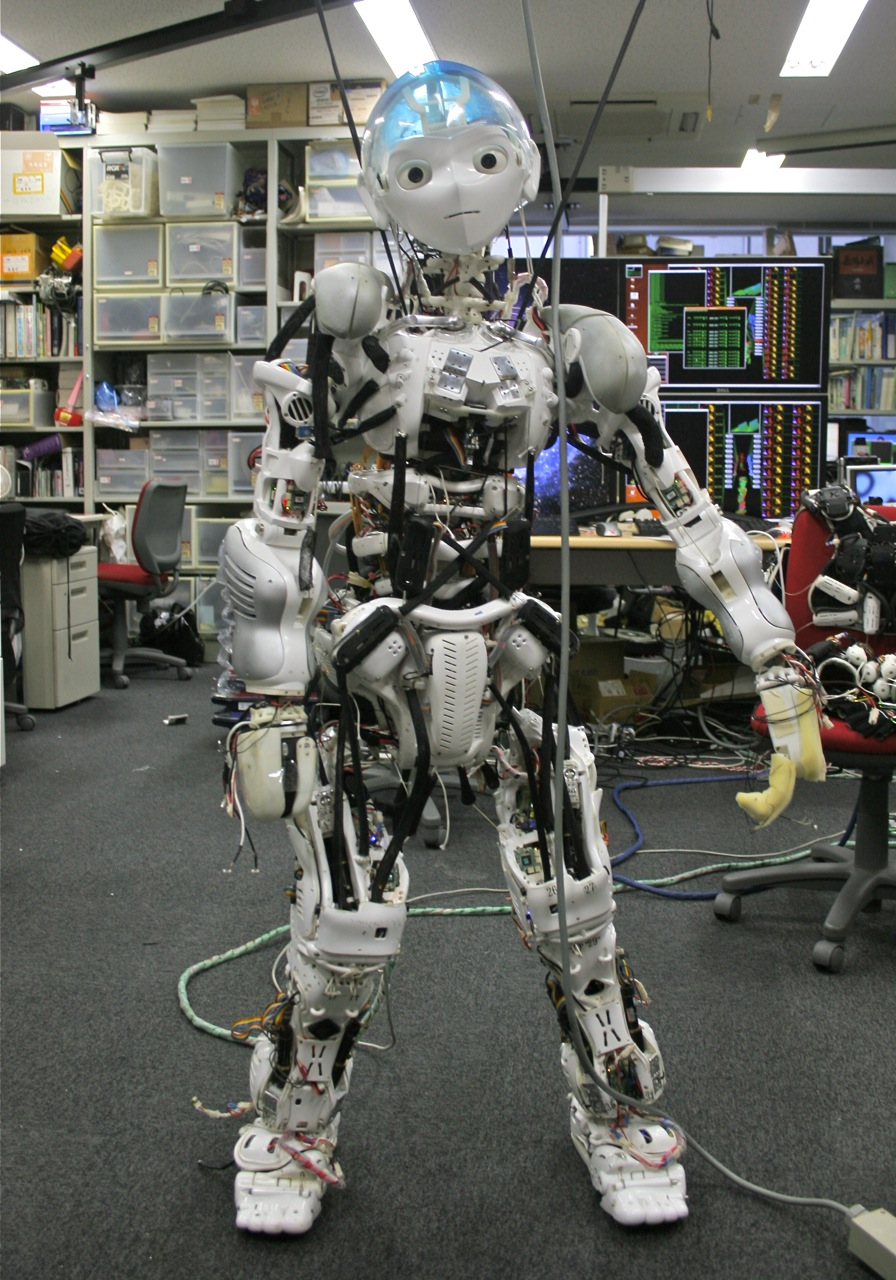
\includegraphics[width=4cm,height=6cm]{chapters/intro/images/kojiro.jpg}}\quad
\end{subfigure}
\begin{subfigure}
[Kenshiro]{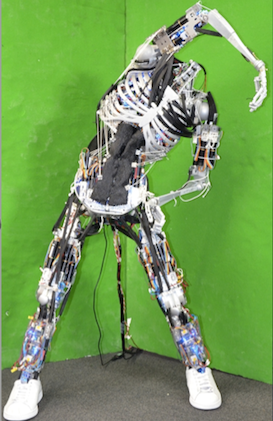
\includegraphics[width=4.1cm,height=6cm]{chapters/intro/images/kenshiro.png}}\quad
\end{subfigure}
\caption{Japanese Humanoids }
\label{fig:hr_second}
\end{figure}

SARCOS Research Corporation and ATR (Advanced Telecommunications Research Institute International) from Japan built robots Erato DB (Dynamic Brain) based on hydraulic actuation in 2000 \cite{atkeson2000using}, and CBi in 2006 \cite{cheng2007cb} which explores the background neural processes in the human brain. DARPA Robotics Challenge (DRC), a competition funded by US Defense Advanced Research Projects Agency (DARPA)  was held between 2012-2015 motivated the development of humanoid robots in the US.  CHARLI in 2010 \cite{knabe2013team}, THOR in 2014 \cite{yi2015team}, CHIMP in 2013 \cite{stentz2015chimp}, Valkyrie in 2013 \cite{radford2015valkyrie} are some popular robots in the US.Most of the robots presented above are fully actuated electrical systems which usually compose rigid bodies with compliance only in the foot to handle contact impacts from the ground while walking. Also they mostly use the traditional high-gain position control methodologies which requires a precise robot dynamic model and Zero Moment Point (ZMP) concept by Vukobratovic \cite{vukobratovic1972stability} is applied in the control of many bipeds \cite{hirai1998development,Kaneko04humanoidrobot,grey2013multi}. 

The advanced robots are expected to make intelligent interactions with the environment. Torque control has gained enough attention in the recent past for its ability to make robust and compliant interactions with the environment and human beings with greater agility and safety. Human safety is one crucial issue which doesn't allow service robots in mobile or humanoid form to be commercialized as domestic robots. Higher compliance brings automatic adaption to un-modeled and uncertain environments making the interaction safer than executing the traditional position control on robots. There are two main categories of torque control: Impedance control and Inverse dynamics control. Impedance Control \cite{part1985impedance,albu2007unified,ott2008passivity,schaffer2008soft} is known for its passivity properties very suitable for interaction with humans and unknown environments. Inverse dynamics(ID) control \cite{del2016implementing,buchli2009compliant,righetti2013optimal} is a highly complex technique which needs a dynamic model and joint torque measurements to control the interactions with the world. This technique provides good trajectory tracking and highly compliant behavior with low feedback gains. The new age ID controllers use quadratic programming(QP) solvers which allow to add constraints such as joint limits, torque bounds, contact force friction cones,center of pressure (CoP) limits which are crucial in humanoid robots. The interest in torque control of humanoid robots lead to new range of robots with torque sensing though it can be estimated in robots with no torques sensors as in HRP-2, iCub, HRP-4 and Asimo, etc.
\begin{figure}[!tbph]
\centering
\begin{subfigure}
[SARCOS]{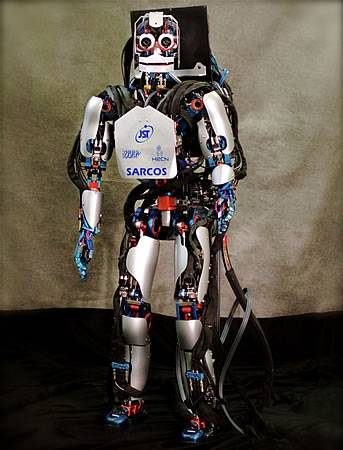
\includegraphics[width=4.2cm,height=6cm]{chapters/intro/images/sarcos.jpg}}\quad
\end{subfigure}
\begin{subfigure}
[CHIMP]{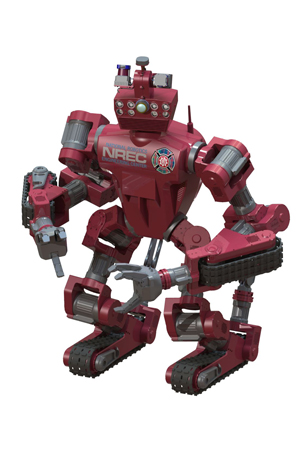
\includegraphics[width=4.2cm,height=6cm]{chapters/intro/images/chimp.jpg}}\quad
\end{subfigure}
\begin{subfigure}
[Valkyrie]{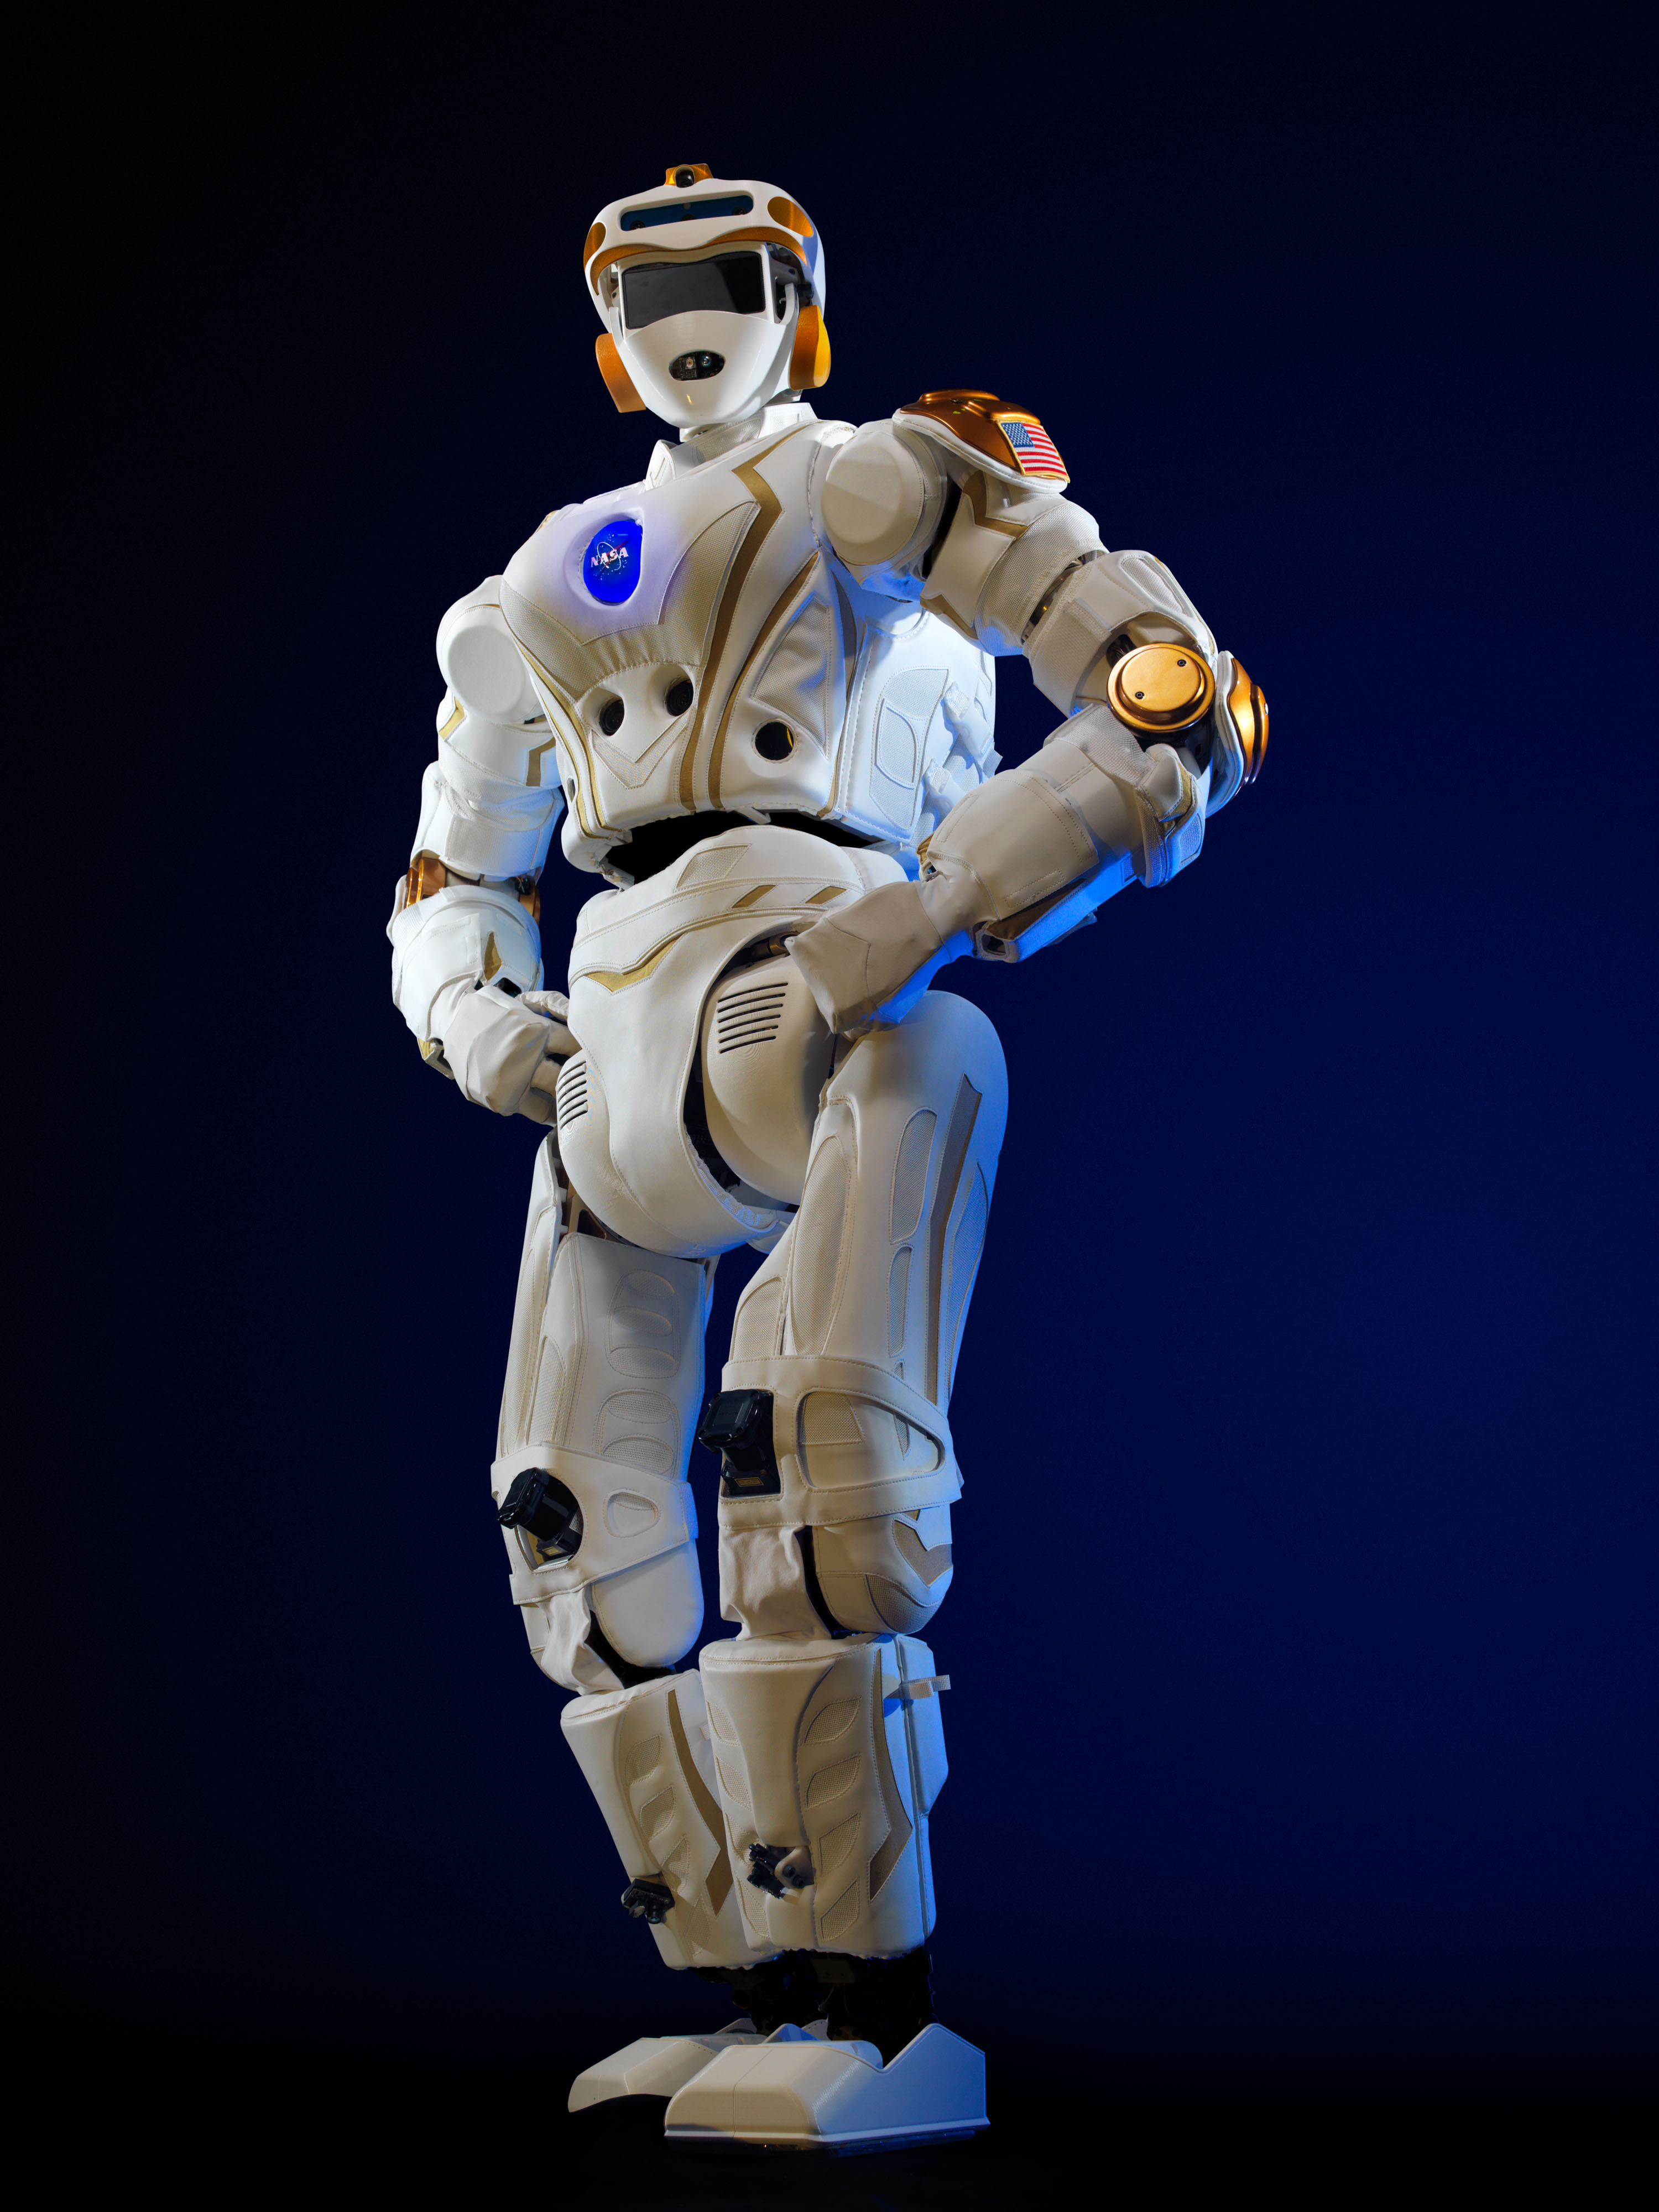
\includegraphics[width=4.2cm,height=6cm]{chapters/intro/images/valkyrie.jpg}}\quad
\end{subfigure}
\caption{Advanced Humanoid Robots}
\label{fig:hr_second}
\end{figure}

 Boston Dynamics built the hydraulics based Petman \cite{nelson2012petman} in 2012 and a series of Atlas robots from 2013. The demonstration video of Atlas in 2016 illustrated the powerful capability of the hydraulic robots by performing tasks which were impossible in the robots of the previous generation. Hydraulic actuation provides high bandwidth and high power density with the price of huge power requirements and noisy hydraulic pumps. High un-modeled friction/stiction makes it harder to control and also the high strength of actuators doesn't allow safe human-robot interaction. Series elastic actuators are also used by some laboratories in their humanoid platforms to implement torque control. The deflections in spring are measured to sense torque, and regulated to execute control on the robot. StarlETH from ETH \cite{hutter2012starleth}, IIT’s COMAN robot \cite{tsagarakis2013compliant}, Human Centered Robotics lab's Hume \cite{slovich2012hume}, IHMC’s M2V2 \cite{pratt2008design}, WALKMAN \cite{negrello2016walk}. Series elastic actuators are mechanical robust, shock absorbing and energy efficient \cite{kormushev2011bipedal} if properly controlled. Moreover, the torque control problem becomes very difficult when the actuators are very compliant and it requires precise modeling of the system dynamics.

Electrical drive units with torque sensors are still a better choice as it is necessary to perform stiff position control in some applications along with the need to have less acoustic noise and low maintenance. DLR's advanced Light Weight Robot (LWR) technology \cite{hirzinger2002dlr} for torque controlled electrical robot arms let them develop the Rollin' Justin, a humanoid upper body and the DLR biped robot \cite{ott2010development}. LWR drives were exploited in such a way it doesn't require any customization to develop a complete humanoid robot specifically for a purpose such as walking or running. TORO, a torque controlled humanoid robot with DLR-Biped legs has abilities to perform multi contact interaction and dynamic whole body motion \cite{englsberger2014overview}. The robot is equipped with torque \& position sensors in the joints including the feet and IMUs in the trunk which makes it appropriate for torque control. DURUS from SRI \cite{hereid20163d} is another robot with torque sensors and a very efficient energy transmission system with high mechanical compliance. Compliance is an important aspect to be considered when it comes to designing humanoid robots. High stiffness is required for tasks such as manipulation and for contact support whereas low stiffness is required for human-robot interaction, walking and for more dynamic activities. Ideally, we need a robot that can handle both these scenarios with ease which leaves with the idea of controlled compliance. 
\begin{figure}[!tbph]
\centering
\begin{subfigure}
[ATLAS]{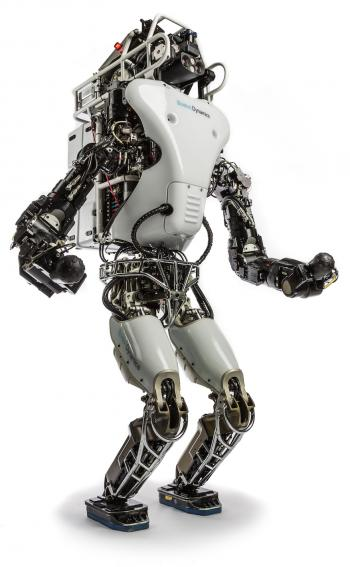
\includegraphics[width=4cm,height=6.5cm]{chapters/intro/images/atlas.jpg}}\quad
\end{subfigure}
\begin{subfigure}
[TORO]{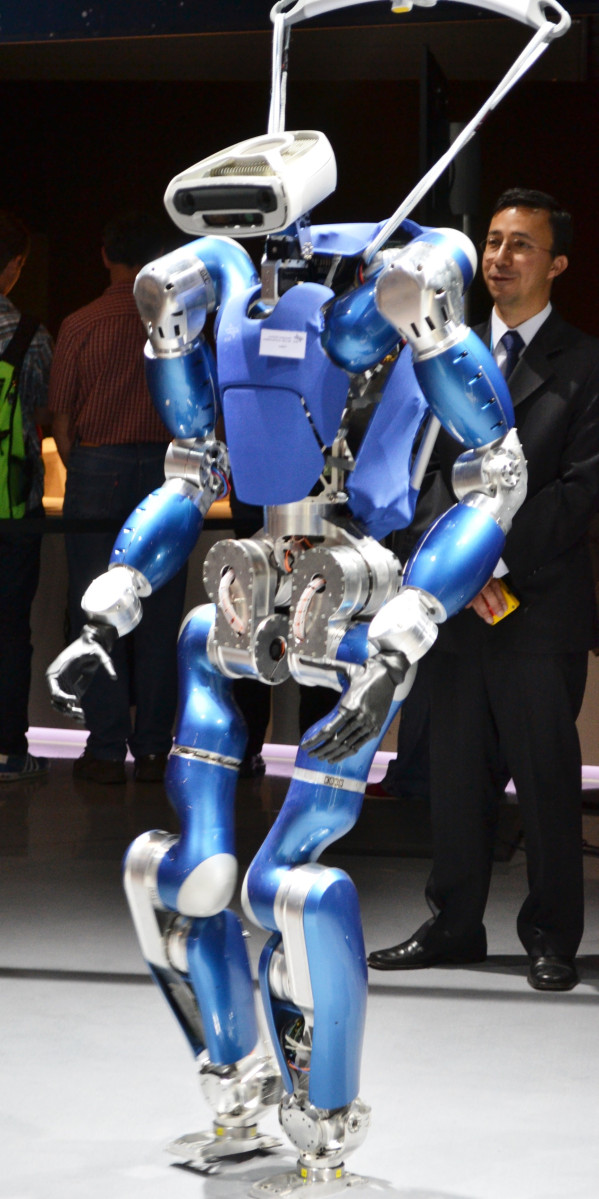
\includegraphics[width=4cm,height=6.5cm]{chapters/intro/images/toro.jpg}}\quad
\end{subfigure}
\begin{subfigure}
[TALOS]{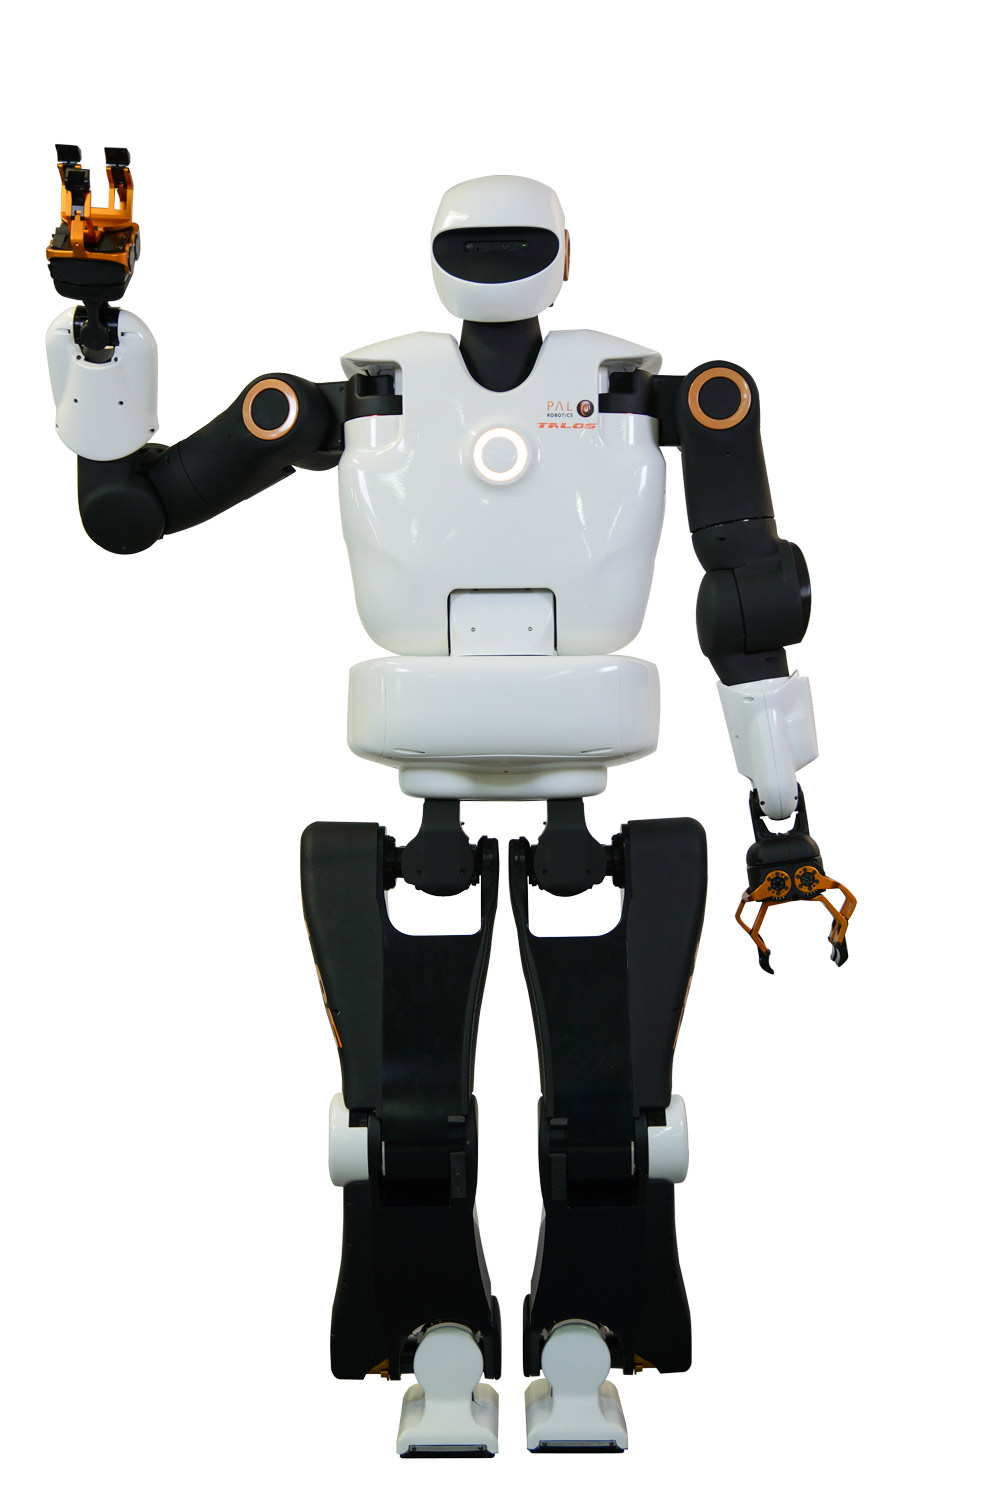
\includegraphics[width=4cm,height=6.5cm]{chapters/intro/images/talos.jpg}}\quad
\end{subfigure}
\caption{Latest Humanoid Robots}
\label{fig:hr_third}
\end{figure}

\subsection{Humanoids in Real Situations}
 Though there are a variety of humanoid robots with a lot of research going on, the applicability of those robots are quite limited. DRC competition challenged the limits of the humanoid robots by putting them in complex scenarios in dangerous environments. It is a great milestone in terms of the amount of attention the competition received and the participation of teams from different places in the world to solve problems in humanoid robotics. After filtering a lot of teams in the DRC simulation, 16 teams managed to contest in the trails. It involves a rich set of tasks that includes driving a utility vehicle, locomote across rubbles, remove debris, manipulate various tools such valves, fire hose and more. TEAM Kaist with their robot DRC-HUBO wont the contest. DRC has shown us how the robots perform in reality in spite of all the technologies working in controlled environment or in simulation. 


\begin{figure}[h]
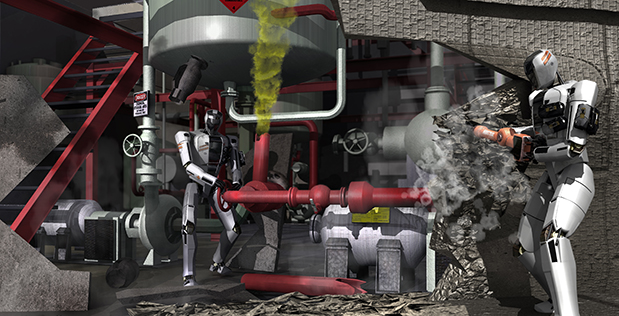
\includegraphics[scale=0.59,right]{chapters/intro/images/darpa.jpg}
\caption{DARPA Robotic Challenge}
\label{fig:darpa}
\end{figure}

The trails showed the lack of capabilities and functional robustness in task scenarios in spite of having tele-operators for guidance. The realization is that the technology is not matured enough and there are a plenty of problems to overcome. There are various aspects to these robot failures.
\begin{itemize}
    \item \textit{Robot Design}: The mechanical design of the robot has influence on the kind of failures it encounters with the environment. Walking on a flat surface is different from rough surfaces and an appropriate mechanical design is necessary to eliminate failures.

    \item \textit{Behavior Design}: The generated behaviors have to be robust to hardware failures. The kind of behaviors we choose have a big influence on the failures as well. This means robot should be able to handle variations in the task making the behavior robust. The whole body motion is also physically not depending on the external contacts. The robots usually have little or no ability to locomote using external contacts. For instance, it is very natural to hold the railings to climb up the stairs which reduces a significant amount of actuation in the joints.
    
    \item \textit{Human Robot Interaction}: When the human wants to control the robot in all the levels and switch between the modes easily, then it is not interaction anymore but intervention. Also trying to perform tasks as soon as possible puts the robot in a dynamic disadvantage.       
 
    \item \textit{Planning and Control}: Humanoid robots are redundant systems with more than 30 degrees of freedom which makes the whole body control complex. Also the pose of the robot can be only controlled indirectly by appropriate joint motions and its interaction with the environment making these robots under-actuated. 
    Constraint based inverse kinematics helps in handling control problems of humanoid robots but it is still challenging to eliminate undesired motions of the rest of the robot links while you execute the intended action in the task space. The physical interaction with the environment makes it more challenging to generate coordinated motions as it creates a variety of structural changes in the kinematics and dynamics of the robot changing the dimension of the problem. Switching control behaviors due to physical contact or joint limits or kinematic singularities challenges the limits of optimization solvers resulting in discontinuities in control. There is an ineffective use of foot torque/force sensors to close the control loop. All these problems make it easy for the robot to lose its balance.   
  
    \item \textit{Error Detection}: It is necessary to eliminate robot falls and they are mostly caused by errors generated by the system itself rather than perturbations from the environment. Detecting errors earlier can give a lot of time to take an appropriate control action to maintain balance. Though there are strategies available to handle external perturbations such as 'Push-Recovery' for example, robot generated errors are given less attention. Aborting the current behavior after detecting errors works but there is a necessity to handle them systematically. 

\end{itemize}

The above aspects shows the practical reality of the humanoid robots and the necessity of various components to function appropriately to be robust to failures. Balancing of legged robots is an essential safety constraint and the ability to handle failures is the motivation to focus on robust  balancing under inertial uncertainties of the robot model.  

\section{Control Methodologies in Humanoid Robotics}
\label{sec:control_methods}
Control methodologies in robotics generally define a control law that allows feasible motion generation with respect to both the robot and environmental constraints to achieve one or multiple desired tasks. There are a variety of methods to generate motion depending upon the robot, the environment and complexity of the task. The control of humanoid robots is quite specific and challenging because of the kinematic redundancy and the dynamic complexity of the system. They have a non-trivial kinematic tree structure with an essential need to stabilize the position of its center of mass(CoM) with respect to the feet at every moment while executing other tasks. In simple words, a humanoid robot cannot walk or run without knowing how to balance itself while in motion. 

Another challenging aspect to be considered here is that the dimension of task space does not equal the dimension of the actuators. Typical tasks consist in controlling the position and orientation of an end-effector (i.e. 6 dimensions), while a humanoid robot has more than 20 degrees of freedom. An inherent task-joint space mapping exists in the form of a trained nervous system in human beings but the robots need a very good dynamic model and appropriate cost functions to make deterministic interactions with the world. Humanoid robots are under-actuated systems which means their pose cannot be controlled directly but by a consequence of commanding appropriate trajectories in joint configuration space. In the following we discuss the state of the art 
approaches used in generating motions.

\subsection{Motion Planning}
Motion planning in robotics refers to the process of searching discrete and feasible motion sequences to achieve a desired task usually satisfying safety constraints and optimal criteria relevant to the task. A motion planning algorithm can be used to plan motion for a variety of tasks ranging from simple arm manipulation for 6 degree of freedom (DoF) robot arms \cite{donald1987search,lozano1987simple} to advanced walking pattern generation for legged robots \cite{kajita2003biped,huang2001planning,harada2006analytical}. The basic idea is to produce continuous motion sequences that connect a start and a goal configuration of the robot while avoiding collision with the obstacles and satisfying certain criteria specific to the task. 
\paragraph{Work Space}
The \textit{Work Space}(\WS) is the set of all robot positions that define the working volume of the robot end effector \cite{cao2011accurate}. This idea can be extended to mobile robot navigation or humanoid locomotion though the definition restricts to end effectors of robot manipulators. The robot and the obstacles are defined in the (\WS) but the motion is always computed or represented in the configuration space, which usually has higher dimension.  

\paragraph{Configuration Space}


The \textit{Configuration Space}(\CS{}) is the set of all configurations a robot can possibly attain. The \CS{} for a robot with \textit{n} degrees of freedom, is a manifold \M{} of \textit{n} dimensions with all robot configurations $q\in$\M{}. The important aspect is that the planning problem in a \WS{} of \sethree{} is transformed to a planning a point motion in its corresponding \CS{}. \CSobst{} represents the robot configurations that are self-colliding or in collision with the environment while \CSfree{} represents its complement. These subspaces allow the planning algorithm to search for a feasible path connecting the start and the end configuration avoiding collisions. 


\paragraph{Algorithms}Over the last 30 years, there has been a lot of research done in motion planning due to the variety of applications . A planning  algorithm is said to be complete if it can find a plan for all the instances of a problem when at least one exists, or report a failure if none exists. Computational complexity  is used to assess the performance of complete planning algorithms. Incomplete planners are not reliable though they are quite effective sometimes in practice. The algorithms can be categorized into \textit{deterministic} and \textit{sampling} based algorithms.
\begin{itemize}
\item \textit{Deterministic Algorithms}: These planning algorithms rely on a deterministic function to compute the path, always resulting in the same motion plan given the same planning request at any instant. Geometric approaches such as visibility graphs, cellular decomposition, Voronoi diagrams and Canny's algorithm compute the shape of \CSfree{} and its connectivity using graphs or road maps \cite{toth2004handbook,canny1988complexity} whereas Grid based approaches represents the configuration space in grids. They use search algorithms(such as $A^*$) to find a path based on the discrete number of actions within \CSfree{} region. These algorithms in general are computationally expensive for high dimensional configuration spaces. Potential field based methods \cite{barraquand1992numerical,koren1991potential} relies on artificially creaing an attractive potential field for the goal and a repulsive field to plan the instantaneous path. The approach is very efficient but it suffers from local minima. Reward based algorithms search for a path that maximizes the cumulative reward constrained by positive reward for reaching a goal and negative reward for collision with obstacles. Markov Decision Processes framework is used in most of the reward-based algorithms generating optimal path \cite{spaan2004point}. 
\item \textit{Sampling based Algorithms}: Sampling based algorithms approximate the connectivity of the feasible configurations in \CSfree{} by random sampling collision free configurations from \CS{} \cite{hudson1997v,gottschalk1996obbtree,hsu1997path}. \textit{Rapidly-exploring Random Trees}(RRT) is a quite popular algorithm which uses Voronoi bias to explore the free configuration space and grows a tree by sampling randomly at every iteration to connect the start and the goal point in \CSfree{}. In a slightly modified version referred to as \textit{Bi-directional RRT}, trees are grown from both the start and goal simultaneously to accelerate the process of the search \cite{kuffner2000rrt}. \textit{Probabilistic Roadmaps}(PRM) randomly sample from the \CS{} and connections are made with the neighbors generated by \textit{k} nearest neighbors or using a local planner \cite{karaman2011sampling}. A road map is developed by adding more configurations and connections until it is dense enough to be used for a planning problem. A path is searched or queried on the generated roadmap using Dijkstra's shortest path algorithm. There are a variety of PRM extensions to achieve better performance \cite{geraerts2004comparative}. Variations such as PRM* and RRT* for generic use cases preserve the asymptotic optimality of the tree \cite{karaman2011sampling}. Kinodynamic RRT* has been proposed for systems with controllable linear dynamics \cite{webb2013kinodynamic} and RRTs have been extended to LQR-Trees in state space \cite{tedrake2010lqr} and LQR-RRT* for linearized systems \cite{perez2012lqr}. Another extension \textit{Transition based RRT} uses stochastic optimization for computing potential states \cite{jaillet2008transition}. Sampling based algorithms deal with high dimensional configuration spaces and are probabilistically complete which means the probability that they fail to provide a solution approaches zero when more time is spent though there is no guarantee if a solution really exists or not.
\end{itemize}


Trajectory optimization is used to reduce the path length while preserving its validity. There are a variety of methods to optimize the trajectory such as greedy optimization \cite{thrun2002probabilistic}  which connects the start and the nearest node configuration that avoids obstacles in an iterative sequence until it reaches the goal configuration. 



\paragraph{Planning in Humanoid Robots}


As discussed before, Humanoid robots are under-actuated and balancing is essential to perform any other meaningful tasks. The motion planning algorithms described previously search for a collision free path considering only the geometry but do not really consider the effects of joint configurations on the whole robot itself. RRT algorithms are able to generate collision-free trajectories but do not optimize their smoothness or the associated control effort. There is a certain amount of control necessary to deterministically choose the right trajectories for tasks specific to a robot and the environment. So in humanoid robots or any polyarticulated system, inverse kinematic/dynamic or optimal control methodology can be used to generate trajectories under constraints. For instance, in humanoid robots it could be necessary to satisfy balance constraints under multiple contact while walking up the steps. In \cite{zhang2014motion}, predefined motion primitives guide the planner to generate natural trajectories.

With regard to Humanoid walking, deterministic planning approaches use a foot transition model with dynamic considerations and the trajectory smoothness during posture transitions \cite{chestnutt2005footstep,ayaz2007human} though there is no guarentee of completeness. Instead probobalistically complete methodologies like RRT can be used to search in discrete footsteps space \cite{perrin2012fast,xia2009random}. Goal-directed approaches such as in \cite{hornung2013search} ensures the path within bounded limits set by the optimal control solutions. Environment features such as contact points can also be used to guide planning \cite{bouyarmane2012dynamics,Escande2013}. There are also some approaches that decompose the problem from higher dimensions into smaller dimensions and are successively solved \cite{zhang2009motion,yoshida2008planning}. Planning is also done on constraint sub-manifolds within \CS{}. Approaches such as in \cite{bretl2006motion,hauser2010multi}, planning is done on union of sub-manifolds defined by balance constraints and leg positions for robots on uneven terrains. In \cite{berenson2011task}, they use jacobian based methods 
to add end effector pose constraints in a \textit{Constrained Bidirectional} RRT planner. In \cite{dalibard2013dynamic}, RRT is adapted within a random diffusion framework to generate statically stable trajectories. In recent times, path planning is combined with optimal contol to generate motion in cluttered environment \cite{el2013optimal}.

\subsection{Kinematic Control}
\paragraph{Basics of Robot Kinematics}
Kinematics is the study of movement of kinematic chains considering the geometry while ignoring the dynamic properties such as mass, inertia of the system and forces or torques to generate motion. The relationship between position, velocity and acceleration of the links of the system with respect to its kinematic connectivity and dimensionality is studied to control the movement of the system in joint space. The joint space of a robot with \textit{n} DoF is an \textit{n} dimensional manifold $\mathcal{Q}$ with all possible joint values. But in robotics, the pose of certain points are important for control in the task space. These point are generalized to \textit{Operational Points} \cite{Khatib1987}. The variation in an operational point x can be represented by a twist $\xi$ comprising linear and angular velocities \cite{featherstone2008rigid,Murray1994}. The kinematic control problem can be defined in four different ways:
\begin{itemize}
    \item \textit{Forward Kinematics}: Given a joint configuration $q \in \mathcal{Q}$, it involves finding the pose of an operational point $x \in SE(3)$ described by $x = f(q)$ such that $f:\mathcal{Q} \rightarrow SE(3)$. Denavit-Hartenberg(DH) parameters \cite{hartenberg1955kinematic} introduced in \cite{craig2005introduction} is quite a popular method used to represent the forward kinematics for serial manipulators though they are not suitable for closed kinematic chains and robot calibration \cite{khalil2004modeling,everett1987kinematic}. Other approaches include the \textit{Khalil-Kleinfinger} notations for closed loop robots \cite{khalil2004modeling}, \textit{Hayati-Roberts} coordinates for avoiding singularities \cite{hayati1985improving, roberts1988new}, screw theory modeling \cite{tsai1999robot}, product of exponentials(PoE) \cite{park1994computational} and methods 
    specific to humanoid robots as in \cite{kajita2005humanoid}.

    \item \textit{Forward differential kinematics}: Given a joint configuration variation $\dot{q} \in T_q(\mathcal{Q})$, it involves finding the twist of an operational point $\xi \in se(3)$ described by  $\xi = J_o(q)\dot{q}$ such that  $J_o:T_q(\mathcal{Q}) \rightarrow se(3)$ where $J_o$ is the tangent or geometric jacobian \cite{spong2006robot,Khatib1987} and $T_q(\mathcal{Q})$ is tangential to $\mathcal{Q}$ at $q$.
    \item \textit{Inverse Kinematics}: Given a pose $x \in SE(3)$ for an operational point, it involves finding the joint configuration
    $ q \in \mathcal{Q}$ described by $q = f^{-1}(x)$ such that $f^{-1}:SE(3) \rightarrow \mathcal{Q} $. The \textit{Inverse Kinematics} problem can be solved analytically for certain kinematic structures either using algebraic approaches as in \cite{paul1robot} \cite{RaghvanBoth1993inverse} or geometric approaches as in \cite{paden1985kinematics, peiper1968kinematics}.

    \item \textit{Inverse differential kinematics}: Given a twist $\xi \in se(3)$ for an operational point, it involves finding the 
    joint velocities $\dot{q} \in T_q(\mathcal{Q})$ described by $ \dot{q} = J_o(q)^{+}\xi$ where $J_o^{+}$ is a pseudo inverse such that $J_o^{+}:se(3) \rightarrow T_q (\mathcal{Q})$. It is solved analytically in \cite{Chiaverini1994,Chiaverini1997,siciliano1999tricept}  

\end{itemize}

\paragraph{Kinematic Redundancy}
The kinematic control involves reaching a reference point or tracking a trajectory in $SE(3)$ for one or more operational points by searching for the appropriate instantaneous joint configurations  $q(t)$. Such goals are called tasks. When the dimensions of the robot $n$ exceeds the task DoF $n_t$, the robot is said to be kinematically redundant with $n − n_t$ being the degree of redundancy with respect to task \cite{nakamura1990advanced}. Though it provides flexibility in the joint space to manage the constraints effectively, it is quite complex to handle the inverse kinematics in a multiple task scenario \cite{siciliano1991general}. Closed form solutions are not possible in redundant robots and choosing a solution that solves both the main and the complementary tasks as much as possible is essential. For instance, it is expected from a robotic arm to manipulate an object while avoiding collisions with the environmental obstacles reactively. Numerical approaches are used to solve these multi-task control problems on redundant robots.

Numerical methods formulate \textit{Inverse Kinematics} as a constrained optimization problem either globally or locally. Global methods search for an optimal path for the entire trajectory which is computational complex \cite{baillieul1990resolution}. Local methods solve them differentially computing locally optimal $dq$ for a small change $dx$ to generate the joint space trajectory $q(t)$. \textit{Resolved Motion Rate Control} in \cite{Whitney1969} finds the $\dot{q}$ by solving the system: $\dot{x} = J(q) \dot{q}$. Damped pseudo inverses \cite{nakamura1986inverse} are used to avoid singularities and inversion issues in redundant robots when the Jacobian is not a full row or column rank matrix. 

 A more generic solution solves each task by projecting onto the nullspace of the Jacobian $J$ supplying certain degrees of freedom to the specific task \cite{Liegeois1977}. There are two ways to carry out the projection systematically.

 \begin{itemize}
     \item \textit{Task Space Augmentation} uses weighting to modulate the task space by constraining the joint space\cite{sciavicco1987solving}. Task conflicts are managed by assigning weights to each task making a compromise between the goals of the tasks.  Proper tuning specific to the scenario is essential for this methodology. \textit{Extended Jacobian Matrix} helps in handling the conflict between tasks by zeroing down the projection of the cost function gradient on the null space of the Jacobian \cite{baillieul1985kinematic}.

     \item \textit{Task Prioritization} strictly prioritizes the projection hierarchically by ensuring that the lower priority task do not affect the tracking error of the higher priority task \cite{nakamura1987task}. A systematic framework for a multi-task scenarios is proposed in \cite{siciliano1991general} which algorithmically generates $\dot{q}$ to minimize the task error in a prioritized way. A solution in \cite{Baerlocher1998} is used to speed up the computation of null space projector. 
     
 \end{itemize}

\paragraph{Redundancy Resolution in Humanoid Robots}
Since humanoids and redundant robots have a tree like structure, closed form solutions are generated by treating the complete robot as a set of many kinematic chains as in \cite{ali2010closed,nunez2012explicit}. These approaches are quite complex and instantaneous inverse kinematic solvers are usually preferred. Linearizing the problem on humanoid robot, produces infinite solutions providing the possibility to perform multiple tasks. \textit{Task Space Augmentation} methods as in \cite{tevatia2000inverse} and \cite{salini2009lqp} suffer from task conflicts resulting in unsuccessful task execution whereas \textit{Task Space Prioritization} has a strict priority on resolving multiple tasks leading to locally optimal results.
 The method is also computationally less expensive and are used in common. Several approaches have been developed for multiple equality constraints at the kinematic level \cite{yoshida2006task,mansard2007task,gienger2005task}. For inequality tasks, sequential quadratic programming is used to solve a cascade of tasks \cite{kanoun2009prioritizing}. A much more efficient implementation using complete orthogonal decomposition
is proposed by \cite{Escande2014} which the state of the art solver Stack of Tasks used to solve a hierarchical quadratic program. \cite{jarquin2013real} also proposes a solution for a smooth transition in control when the priorities are interchanged.  


\subsection{Dynamic Control}

\paragraph{Basics of Robotic Dynamics}
Dynamics is the study of the dynamic relationship between the motion of the kinematic chain and the generalized forces acting on the system to make movement. The generalized forces are the external forces applied to the system which include the joint torques for rotational joints, joint forces for prismatic joints, and also the force due to external contacts. This relationship allows to control the robot in a dynamic level enabling a better interaction with the environment. Dynamic parameters such as length, mass, inertia of the links and the forces or torques acting on the mechanical system are considered. In a robot dynamic model, the motion is defined by joint  acceleration $\ddot{q}$ and operational point acceleration $\ddot{x}$ in the task space. 

\begin{itemize}
    \item \textit{Forward Dynamics} determines the acceleration of the robot in the joint space when generalized forces are applied in the joint space
    \item \textit{Inverse Dynamics} determines the generalized forces necessary in joint space to achieve a required acceleration in the joint space.
\end{itemize}

The two main approaches to model the robot dynamics are:

\begin{itemize}
    \item \textit{Lagrange Method} is energy based with dynamic equations in closed form. \cite{uicker1969dynamic,kahn1969near,bejczy1974robot} are such approaches in the robotics domain. It has a clear separation of each component but it is very expensive  for implementing control schemes. \cite{hollerbach1980recursive} presents an efficient formulation but still \textit{Newton-Euler Method} are preferred for faster computation.
    \item \textit{Newton-Euler Method} is a generalized force based and recursive in nature. The first of its kind is presented in \cite{orin1979kinematic}. It does not clearly separate components but it is computationally cheaper. \cite{Featherstone2009} explains the most common algorithms such as the composite-rigid-body algorithm (CRBA), the articulated-body algorithm (ABA), the recursive Newton-Euler Algorithm (RNEA). 
\end{itemize}
\cite{spong1992remarks} uses an hamiltonian approach for the analysis of the robot dynamics and there exist certain numerical methods to integrate hamiltonian equations efficiently. Alternatively, \textit{Centroidal dynamics} \cite{orin2013centroidal,orin2008centroidal} models the dynamics of the CoM of the robot capturing the constraints imposed by contact forces on the CoM making the dynamic model very simple. But it does not include joint position and torque limits which makes the model approximate failing to describe the angular momentum of the robot. Humanoids walk with very little angular momentum and is set to zero applying when \textit{Centroidal dynamics} .
In contrast to the classic joint space formulation, the operational space formulation \cite{Khatib1987} defines the motion using the task space acceleration, which requires the forces to be formulated as generalized forces in the task space.

\paragraph{Dynamic Control in Humanoid Robotics}
As discussed already, classical techniques are not appropriate for humanoid robots as the control scheme has to execute coordinated motion keeping into account the interaction forces exchanged with the environment along with balance all the time. Stability criteria that constrain the CoM or the zero moment point (ZMP) within the support polygon are often enforced in the controller \cite{wieber2002stability}. A constraint on the ZMP is equivalent to a constraint on the tangential moment at the contact surfaces. The interaction of legs on the ground along with other contacts of the robot body with the environment is also necessary. The contact forces are transformed to generalized forces on the joints which can be controlled only using joint torque control. Dynamic control is quite essential in ensuring motion feasibility, agility and balance in 
humanoid robots.

The operational-space inverse-dynamics (OSID), a generic framework  establishes the whole-body control considering balance, contacts and other constraints. \cite{Khatib2004} proposes a multi-task formulation with sequential projection on  the nullspaces of the tasks at each level. Strict hierarchy allows lower priority tasks not to affect the higher priority tasks. An equivalent approach \cite{mistry2010inverse} uses orthogonal decomposition and kinematic projections to simply control when switching contact constraints and avoids the inversion of mass matrix. \cite{Righetti2011a,Righetti2011} proposes an improved version constraining the ground reaction forces with the friction boundaries. Inequality constraints can not be added in this framework which is quite necessary to implement collision avoidance, joint limits and visual servoing task. OSID's are used within optimization based methodologies to find optimal solutions. Quadratic Programming (QP) based approaches are more popular for redundant systems which allows both equality and inequality tasks. Weighting schemes are used in a QP based approach which provides robust balance \cite{collette2008robust}. \cite{Salini2011} implements a weighting focused on the task prioritization. Decoupling of the dynamics in holonomic and non-holonomic part is used in a QP to generate feasible whole body trajectories \cite{bouyarmane2012dynamics,wieber2006holonomy}. \cite{herzog2013experiments} uses active set method to implement a torque control of the lower part of the robot. OSID in a strictly prioritized QP framework is implemented in \cite{Saab2013}. 


The previous approaches focused on the robot dynamics but the angular momentum was not controlled specifically which is an important part of motion in human beings doing agile and complex motion \cite{popovic2004angular}. \cite{kajita2003resolved} proposed to control the angular momentum of the robot using the inverse of the inertia matrix. \textit{Centroidal dynamics} controls the angular momentum as in \cite{hofmann2009exploiting} focusing on gait movements and \cite{moro2013attractor} where an attractor is used to control. Also \cite{wensing2013generation} uses conic optimization techniques to control the angular momentum generating complex motions.

\subsection{Optimal Control}
Optimal Control involves finding control laws for a given system such that certain optimality criteria are minimized. It is a problem of searching trajectories that satisfy the system dynamics and minimizing a cost function. In Robotics, it is also called as \textit{Trajectory Optimization} or \textit{Trajectory Filtering}.

\paragraph{Background}
Optimal Control is actually an extension of a theory of \textit{Calculus of Variations} that uses optimization methodologies to find control policies. The first ever optimal control solution was proposed for the brachystochrone problem in Bernouli's work. Though there were early contributions to the theory of optimal control by Newton, Euler, Leibniz, Jacobi, Hamilton, Bolza and many others, the formalization began to take shape with the introduction of Linear Quadratic Control(LQC) problem minimizing a squared error of an expected value of a random variable x \cite{wiener1949extrapolation}. The next milestone was the birth of Dynamic Programming (DP) to solve discrete time optimal control problems which reduces the search to Hamilti-Jacobian equation. The formulation of the Pontryagin maximum principle \cite{pontryagin1987mathematical} completely formalize the problem based on the calculus of variations considering  pathwise constraints on control values of the functions. \textit{Linear Quadratic Regulator (LQR)} and the \textit{Linear Quadratic Gaussian (LQG)} are formulated to design optimal control policies in \cite{Kalman1960} which marks another important formulation in optimal control.

\textit{Model Predictive Control (MPC)} also called as Receding Horizon Control is a popular automatic control methodlogy in industries which uses the optimal control solution at each instant over a time horizon called the prediction horizon \cite{richalet1978model}. Task specific goals are specified by simple penalty functions in the optimal control which synthesizes the motion behaviour and control laws. The controller predicts the futures states under certain criteria which lets them find the control values to achieve the appropriate current state avoiding extensive exporation. \textit{Differential Dynamic Programming(DDP)} is a numerical scheme quite efficient for direct implicit optimal control generating local trajectories \cite{jacobson1968new}. A hybrid method uses constant local controllers \cite{atkeson1994using} which is improvized in \cite{atkeson2003nonparametric} using second order local models to make linear controllers.


\paragraph{Optimal Control in Humanoid Robotics}
For humanoid robot walking, the \textit{Operational Space Inverse Dynamics} or \textit{Inverse Kinematics} cannot really handle the accelerations of the CoM properly thus generating very conservative or over restricted motion. Optimal control can find 
trajectories from initial to final posture specified as one complete objective or many objectives with certain constraints. Optimal control can generate proper and powerful trajectories for CoM unlike IK or OSID. It is quite equivalent to a classical walking pattern generator in addition to the ability to incorporate whole body motion. MPC's are a quite relevant control scheme in humanoid robotics and control solutions as in \cite{kajita2003biped,herdt2010online} uses a dedicated Linearize Inverted Pendulum model to predict the future state of the system for controlling dynamic stability. Though it is quite complex and the models have to be created for every new case, optimal control is very appropriate and takes care of all the constraints at the same horizon. One problem with using optimal control in humanoid robotics is the computational time because of more DoFs and it requires a faster response when controlled in dynamic level.

In multiple task scenarios, weighted average of tasks can be used to influence the priority by choosing right weights for each task in the set \cite{dimitrov2011sparse}. It obviously introduces task conflicts if the relative difference of the weights are not significantly high. Large weights can also produce numerical errors resulting in pracitcal complexity to implement such control schemes. In \cite{del2014prioritized}, the optimal control is strictly prioritized avoding such issues. MuJoCo is a state of the art simulator that uses MPC to generate humanoid trajectories with high computational speed with respect to dynamic derivatives\cite{todorov2012mujoco}. Behaviours like getting up from the ground and avoiding disturbances were generated in this simulator \cite{tassa2012synthesis}.  The use of environment increases the controllable space to successively acheive the goals as in \cite{lengagne2013generation} generating non-coplanar contact motions. Parkour motion\cite{dellin2012framework}, kicking a ball \cite{miossec2006development} and  lifting weights \cite{arisumi2008dynamic} shows some application of optimal control in generating complex behaviours.

Variants of DDP exist with respect to optimal control in humanoid robots. Control-limited DDP allows adding inequality constraints as proposed in \cite{tassa2014control}  has been applied on a humanoid robot in simulation. Square-root DDP proposed in \cite{geoffroy2014inverse} shows that IK and OSID are special cases of optimal control without preview horizon. DDP is also used in generating sample trajectories to learn a neural network based guided policy to avoid local minima in \cite{Levine2012}. Behaviors such as walking, running, hopping and swimming are generated using this approach. Robust walking behaviours were generated using DP in \cite{whitman2013coordination} relying on multi model and learning based DP variants. Steep climbing motion is generated in \cite{Noda2014}
which uses Body Retention Load Vector to model the physical constraints. Optimal control has also been treated as an offline control problem in \cite{schultz2010modeling} optimizing energy based criteria using multiple shooting approach to generate running behaviors. Walking motions are generated without using a pattern generator but just by optimizing joint velocities, torques or ZMP constraints \cite{el2013optimal,koch2012studying}. Inverse optimal control involves learning the criteria to generate observed motions in a dynamic system. Human locomotion is studied using inverse optimal control in one such work \cite{mombaur2010human}. Also human running is studied in different terrains and distirubances in \cite{park2013inverse}


Motion planning is also combined with optimization for collision free navigation in a cluttered environment. Motion planners for high DoF systems generate trajectory in two stages: planning and optimization. There are three well known and similar techniques in this domain. CHOMP (Covariant Hamiltonian Optimization for Motion Planning) uses covariant gradient descent technique in the solver resulting in a planning algorithm completely relying on trajectory optimization \cite{zucker2013chomp}. Starting with a naive trajectory, CHOMP optimizes the dynamics of the trajectory while reacting to the obstacles in the environment. STOMP (Stochastic Trajectory Optimization for Motion Planning) is very similar except for the use of trajectory stochastic perturbations to generate trajectories without computing the jacobian \cite{kalakrishnan2011stomp}. ITOMP (Incremental Trajectory Optimization for Real-Time Replanning in Dynamic Environments) can produce suboptimal solutions because of the time constraints on the solver and the trajectory is incrementally updated online \cite{park2014high}.

High dimensionality is challenging in humanoid robotics to get optimal control working in real time. The state space gets large due to high number of DoFs and it is not easy to explore all of it apriori and generate appropriate trajectories for every cases. Current optimal control solutions are time consuming and encounters numerical problems which is sill an open issue in robotics.

\section{Chapter Organization}
The thesis has two main chapters \ref{chapter:framework} and \ref{chapter:rc} describing the two main contributions of this thesis respectively. Chapter \ref{chapter:framework} presents the dynamic obstacle framework developed on industrial robots for collision avoidance using proximity information from skin sensors and point cloud information from 3d cameras. The Chapter \ref{chapter:rc} presents the strategy used to model inertial uncertainties to perform robust balancing. Chapter 5 concludes the thesis with important comments on the contributions and the possible future work connected to it.
\section{Publications}
\begin{itemize}
\item Giftsun, N., Prete, A. Del, \& Lamiraux, F. (2017). \textit{Robustness to Inertial Parameter Errors for Legged Robots Balancing on Level Ground.} International Conference on Informatics in Control, Automation and Robotics (ICINCO) \textbf{[CONFERENCE]}.
\item Bharatheesha, M., Giftsun, N., Hernandez, C., Bergner, F., Dean-leon, E., \& Cheng, G. (2017). \textit{Dynamic Obstacle Avoidance for Collaborative Robot Applications.} IEEE International Conference on Robotics and Automation (ICRA)\textbf{[WORKSHOP]}.
\end{itemize}
\ifdefined\included
\else
\bibliographystyle{acm}
\bibliography{These}
\end{document}
\fi